%%%%%%%%%%%%%%%%%%%%%%%%%%%%%%%%%%%%%%%%%
% Jacobs Landscape Poster
% LaTeX Template
% Version 1.1 (14/06/14)
%
% Created by:
% Computational Physics and Biophysics Group, Jacobs University
% https://teamwork.jacobs-university.de:8443/confluence/display/CoPandBiG/LaTeX+Poster
% 
% Further modified by:
% Nathaniel Johnston (nathaniel@njohnston.ca)
%
% This template has been downloaded from:
% http://www.LaTeXTemplates.com
%
% License:
% CC BY-NC-SA 3.0 (http://creativecommons.org/licenses/by-nc-sa/3.0/)
%
%%%%%%%%%%%%%%%%%%%%%%%%%%%%%%%%%%%%%%%%%

%----------------------------------------------------------------------------------------
%	PACKAGES AND OTHER DOCUMENT CONFIGURATIONS
%----------------------------------------------------------------------------------------

\documentclass[final]{beamer}

\usepackage[scale=1.24]{beamerposter} % Use the beamerposter package for laying out the poster

\usetheme{confposter} % Use the confposter theme supplied with this template

\setbeamercolor{block title}{fg=ngreen,bg=white} % Colors of the block titles
\setbeamercolor{block body}{fg=black,bg=white} % Colors of the body of blocks
\setbeamercolor{block alerted title}{fg=white,bg=dblue!70} % Colors of the highlighted block titles
\setbeamercolor{block alerted body}{fg=black,bg=dblue!10} % Colors of the body of highlighted blocks
% Many more colors are available for use in beamerthemeconfposter.sty

%-----------------------------------------------------------
% Define the column widths and overall poster size
% To set effective sepwid, onecolwid and twocolwid values, first choose how many columns you want and how much separation you want between columns
% In this template, the separation width chosen is 0.024 of the paper width and a 4-column layout
% onecolwid should therefore be (1-(# of columns+1)*sepwid)/# of columns e.g. (1-(4+1)*0.024)/4 = 0.22
% Set twocolwid to be (2*onecolwid)+sepwid = 0.464
% Set threecolwid to be (3*onecolwid)+2*sepwid = 0.708

\newlength{\sepwid}
\newlength{\onecolwid}
\newlength{\twocolwid}
\newlength{\threecolwid}
\setlength{\paperwidth}{48in} % A0 width: 46.8in
\setlength{\paperheight}{36in} % A0 height: 33.1in
\setlength{\sepwid}{0.024\paperwidth} % Separation width (white space) between columns % 0.024 
\setlength{\onecolwid}{0.22\paperwidth} % Width of one column
\setlength{\twocolwid}{0.464\paperwidth} % Width of two columns
\setlength{\threecolwid}{0.708\paperwidth} % Width of three columns
\setlength{\topmargin}{-1in} % Reduce the top margin size -.5
%-----------------------------------------------------------

\usepackage{graphicx}  % Required for including images
\usepackage{booktabs} % Top and bottom rules for tables
\usepackage[font=scriptsize, labelfont=bf]{caption}
\usepackage{subcaption}

\graphicspath{ {../figures/} }

\newcommand{\ind}[1]{1_{#1}} % Indicator function
\newcommand{\pr}{P} % Generic probability
\newcommand{\ex}{E} % Generic expectation
\newcommand{\var}{\textrm{Var}}
\newcommand{\cov}{\textrm{Cov}}
\newcommand{\sgn}{\textrm{sgn}}
\newcommand{\sign}{\textrm{sign}}
\newcommand{\kl}{\textrm{KL}} 
\newcommand{\abs}[1]{|{#1}|}



\renewcommand{\S}{\Sigma}
\renewcommand{\L}{\Lambda}
\renewcommand{\[}{\begin{equation}}
\renewcommand{\]}{\end{equation}}
\renewcommand{\b}{\backslash}
\newcommand{\g}{\,\vert\,}
\newcommand{\tr}{\mathrm{tr}}
\newcommand{\diag}{\mathrm{diag}}
\newcommand{\bea}{\begin{eqnarray}}
\newcommand{\eea}{\end{eqnarray}}
\newcommand{\hx}{\hat{x}}
\newcommand{\hxi}{\hat{\xi}}
\newcommand{\Var}{\mathrm{Var}}
\newcommand{\Cov}{\mathrm{Cov}}
\newcommand{\prop}{\propto}
\newcommand{\deq}{:=}

\newcommand{\EE}{\mathbb{E}}
\newcommand{\II}{\mathbb{I}}
\newcommand{\R}{\mathbb{R}}
\newcommand{\PP}{\mathbb{P}}

\newcommand{\La}{\mathcal{L}}

\newcommand{\n}{\mathcal{N}}

\newcommand{\bx}{\mathbf{x}}
\newcommand{\bX}{\mathbf{X}}
\newcommand{\by}{\mathbf{y}}
\newcommand{\bs}{\mathbf{s}}
\newcommand{\bn}{\mathbf{n}}
\newcommand{\br}{\mathbf{r}}
\newcommand{\bt}{\mathbf{t}}

\newcommand{\fig}[1]{Figure~\ref{fig:#1}}
\newcommand{\chap}[1]{Chapter~\ref{chap:#1}}
\newcommand{\mysec}[1]{Section~\ref{sec:#1}}
\newcommand{\app}[1]{Appendix~\ref{sec:#1}}
\newcommand{\eq}[1]{Eq.~(\ref{eq:#1})}
\newcommand{\eqs}[1]{Eqs.~(\ref{eq:#1})}
\newcommand{\eqss}[1]{(\ref{eq:#1})}
\newcommand{\thm}[1]{Theorem~\ref{thm:#1}}

\newcommand{\indep}{{\;\bot\!\!\!\!\!\!\bot\;}}
\newcommand{\eps}{\varepsilon}

\newcommand{\one}{1}
\newcommand{\Dir}{{\rm Dir}}
\newcommand{\Mult}{{\rm Mult}}
\newcommand{\Bin}{{\rm Bin}}
\newcommand{\Ga}{{\rm Ga}}
\newcommand{\IG}{{\rm IG}}
\newcommand{\InvGa}{{\rm IG}}
\newcommand{\Chisquare}{\Chi^2}
\newcommand{\St}{{\rm St}}
\newcommand{\Beta}{{\rm Beta}}
\newcommand{\iid}{i.i.d.}
\newcommand{\Eta}{{\cal N}}
\newcommand{\Ber}{{\rm Ber}}

\newcommand{\simiid}{\stackrel{\tiny\text{iid}}{\sim}}
\newcommand{\simind}{\stackrel{\tiny\text{ind}}{\sim}}

\DeclareMathOperator*{\BP}{BP}
\DeclareMathOperator*{\DP}{DP}
\DeclareMathOperator*{\GP}{GP}
\DeclareMathOperator*{\BeP}{BeP}

% Caligraphic alphabet
\newcommand{\calr}{\mathcal{R}} % only because \cr already taken
\newcommand{\ca}{\mathcal{A}} \newcommand{\cb}{\mathcal{B}} \newcommand{\cc}{\mathcal{C}} \newcommand{\cd}{\mathcal{D}} \newcommand{\ce}{\mathcal{E}} \newcommand{\cf}{\mathcal{F}} \newcommand{\cg}{\mathcal{G}} \newcommand{\ch}{\mathcal{H}} \newcommand{\ci}{\mathcal{I}} \newcommand{\cj}{\mathcal{J}} \newcommand{\ck}{\mathcal{K}} \newcommand{\cl}{\mathcal{L}} \newcommand{\cm}{\mathcal{M}} \newcommand{\cn}{\mathcal{N}} \newcommand{\co}{\mathcal{O}} \newcommand{\cp}{\mathcal{P}} \newcommand{\cq}{\mathcal{Q}} \newcommand{\cs}{\mathcal{S}} \newcommand{\ct}{\mathcal{T}} \newcommand{\cu}{\mathcal{U}} \newcommand{\cv}{\mathcal{V}} \newcommand{\cw}{\mathcal{W}} \newcommand{\cx}{\mathcal{X}} \newcommand{\cy}{\mathcal{Y}} \newcommand{\cz}{\mathcal{Z}}

% Convergence
\newcommand{\convd}{\stackrel{d}{\longrightarrow}} % convergence in distribution/law/measure
\newcommand{\convp}{\stackrel{P}{\longrightarrow}} % convergence in probability
\newcommand{\convas}{\stackrel{\textrm{a.s.}}{\longrightarrow}} % convergence almost surely
\newcommand{\convr}{\stackrel{r}{\longrightarrow}} % convergence in r^{th} mean

\newcommand{\eqd}{\stackrel{d}{=}} % equal in distribution/law/measure
\newcommand{\argmax}{\mathop{\mathrm{argmax}}}
\newcommand{\argmin}{\mathop{\mathrm{argmin}}}
\newcommand{\conv}{\textrm{conv}} % for denoting the convex hull


\makeatletter
\providecommand*{\diff}%
	{\@ifnextchar^{\DIfF}{\DIfF^{}}}
\def\DIfF^#1{%
	\mathop{\mathrm{\mathstrut d}}%
		\nolimits^{#1}\gobblespace}
\def\gobblespace{%
	\futurelet\diffarg\opspace}
\def\opspace{%
	\let\DiffSpace\!%
	\ifx\diffarg(%
		\let\DiffSpace\relax
	\else
		\ifx\diffarg[%
			\let\DiffSpace\relax
	\else
		\ifx\diffarg\{%
			\let\DiffSpace\relax
		\fi\fi\fi\DiffSpace}


\providecommand*{\deriv}[3][]{\frac{\diff^{#1}#2}{\diff #3^{#1}}}
\providecommand*{\pderiv}[3][]{\frac{\partial^{#1}#2}{\partial #3^{#1}}}
		
\newcommand{\threequals}{\equiv}
%----------------------------------------------------------------------------------------
%	TITLE SECTION 
%----------------------------------------------------------------------------------------

\title{Latent Community Detection for Modeling Legislative Roll Call Votes} % Poster title

\author{Eli Ben-Michael, Runjing Liu, Jake Soloff } % Author(s)

\institute{Department of Statistics, UC Berkeley} % Institution(s)

%----------------------------------------------------------------------------------------

\begin{document}




\addtobeamertemplate{block end}{}{\vspace*{2ex}} % White space under blocks
\addtobeamertemplate{block alerted end}{}{\vspace*{2ex}} % White space under highlighted (alert) blocks

\setlength{\belowcaptionskip}{2ex} % White space under figures
\setlength\belowdisplayshortskip{2ex} % White space under equations

\begin{frame}[t] % The whole poster is enclosed in one beamer frame

%\begin{picture}(2850,-75)
%\put(0,0){\hbox{
\includegraphics[scale=0.3]{berkeleylogo.jpg}}}
%\end{picture}


\begin{columns}[t] % The whole poster consists of three major columns, the second of which is split into two columns twice - the [t] option aligns each column's content to the top

\begin{column}{\sepwid}\end{column} % Empty spacer column

\begin{column}{\onecolwid} % The first column

%----------------------------------------------------------------------------------------
%	OBJECTIVES
%----------------------------------------------------------------------------------------



\begin{alertblock}{Objectives}
We analyze voting data in the House of Representatives during the 110th Congress (2007-2008). We extend an ideal point model to incorporate caucus membership data via a stochastic block model. In doing so, we aim to 
\begin{itemize}
\item Use caucus membership data to infer latent communities among representatives.
\item Exploit this community structure to inform an estimate for each representative's ideal point.
\item Model a representative's voting behavior.
\end{itemize}

\end{alertblock}

%----------------------------------------------------------------------------------------
%	INTRODUCTION
%----------------------------------------------------------------------------------------

\begin{block}{Motivation}
%Simple dimensionality techniques on roll call votes enable visualization of the voting behavior among the representatives; these techniques are able to detect coarse patterns such as party affiliation. 
%\begin{figure}[h]
%  \centering
%    \begin{subfigure}[b]{0.49\textwidth}
%        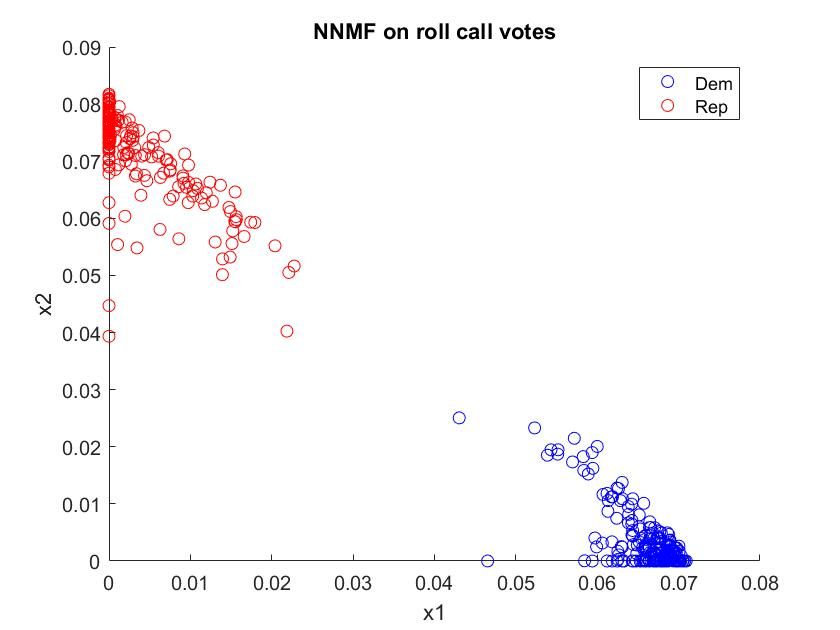
\includegraphics[width=\textwidth]{NNMF_votes.jpg}
%        \caption{}
%        \label{fig:NNMF}
%    \end{subfigure}
%          \begin{subfigure}[b]{0.49\textwidth}
%        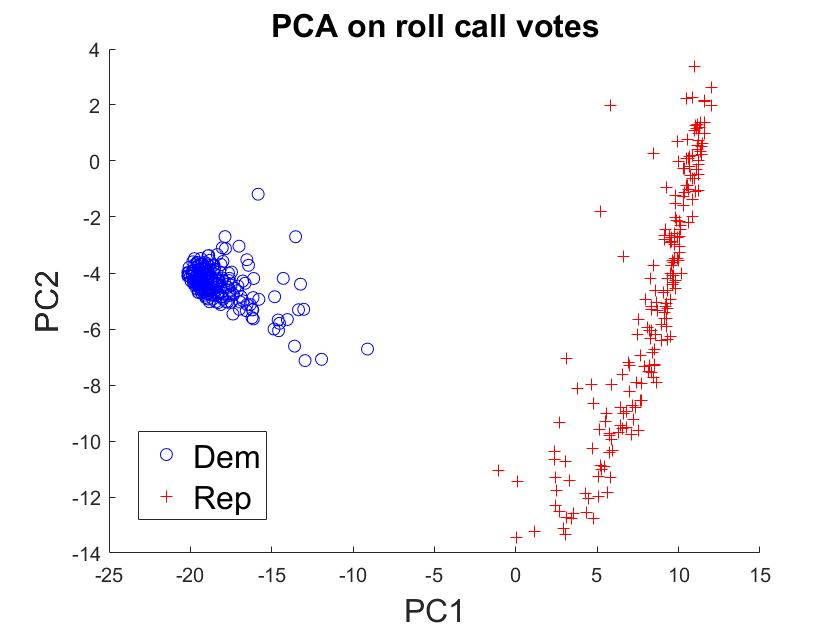
\includegraphics[width=\textwidth]{PCA_votes}
%        \caption{}
%        \label{fig:PCA}
%    \end{subfigure}
%  \caption{(a) Nonnegative matrix factorization on the $448\times 1707$ matrix of roll call vote data (448 representatives, 1707 bills) (b) Principle component analysis on the roll call vote data}
%\end{figure}
We model caucus membership because we found that caucus memberships influence legislative behavior. For example, the more caucuses two legislators share, the more likely they are to vote the same way on a bill. 

\begin{figure}[h]
  \centering
        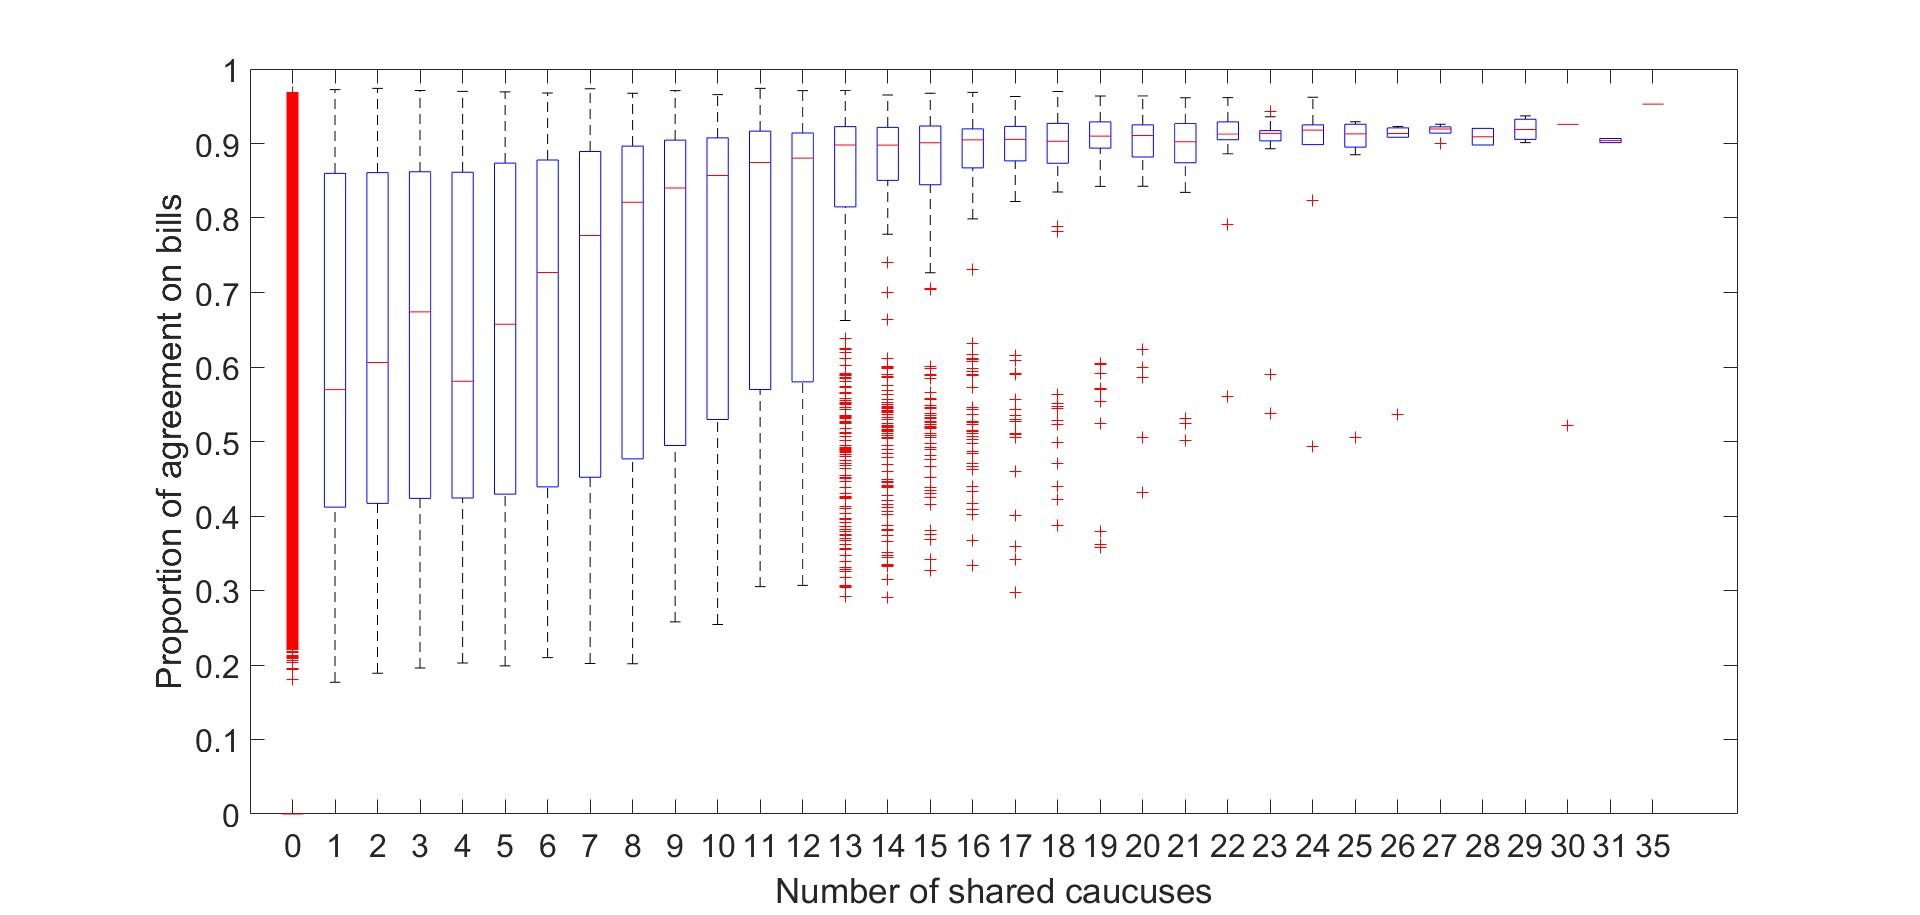
\includegraphics[width=\textwidth]{Caucus_vs_Votes.jpg}
  %\caption{The distribution of agreement on bills as a function of the number of caucuses two representatives share. We see that the more caucuses people share, the more likely they are to agree on a bill. }
         % \label{fig:VotesVsCaucus}
\end{figure}


We used neighborhood selection on roll call vote data to represent interactions among members of the House as an undirected graphical model; we found that subgraphs corresponding to caucuses were denser than the graph of the whole House. 



\begin{figure}[h]
  \centering
    \begin{subfigure}[b]{0.49\textwidth}
        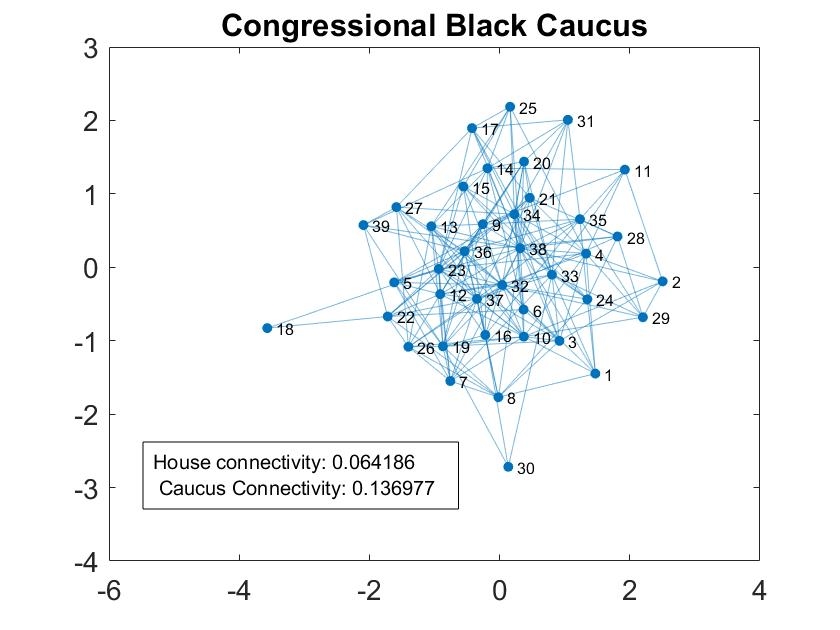
\includegraphics[width=\textwidth]{/Neighborhood_Regression/Congressional_Black_Caucus.jpg}
    \end{subfigure}
          \begin{subfigure}[b]{0.49\textwidth}
        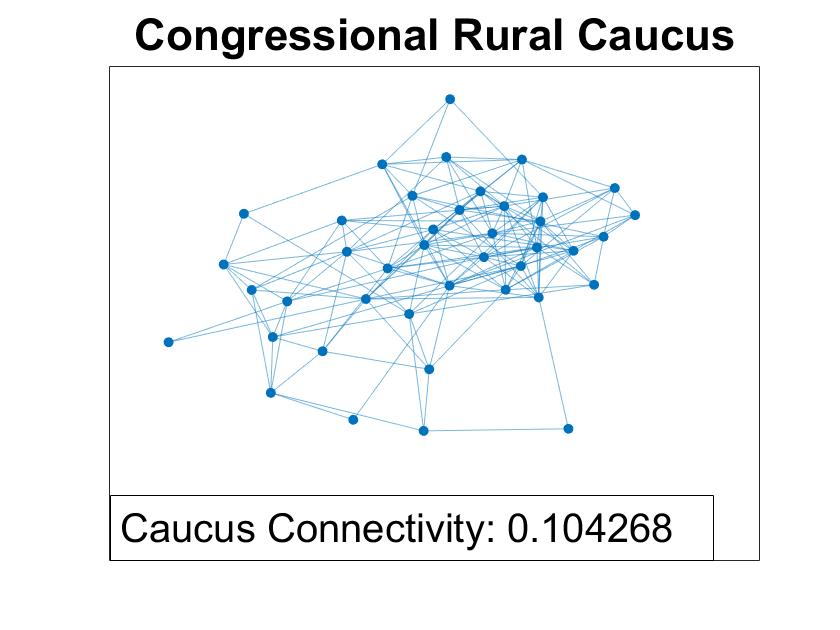
\includegraphics[width=\textwidth]{/Neighborhood_Regression/Congr_Rural_Caucus.jpg}
    \end{subfigure}
        \begin{subfigure}[b]{0.49\textwidth}
        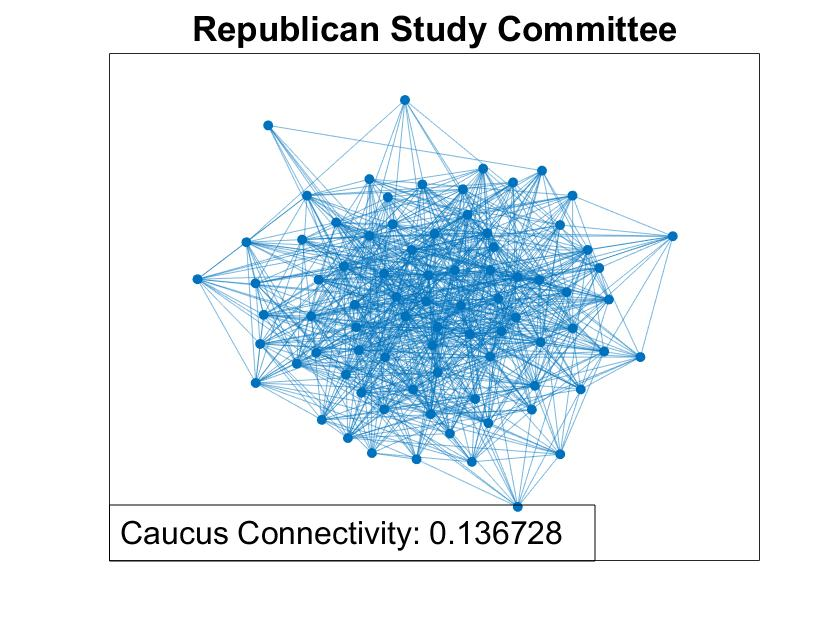
\includegraphics[width=\textwidth]{/Neighborhood_Regression/Rep_Study_Committee.jpg}
    \end{subfigure}
          \begin{subfigure}[b]{0.49\textwidth}
        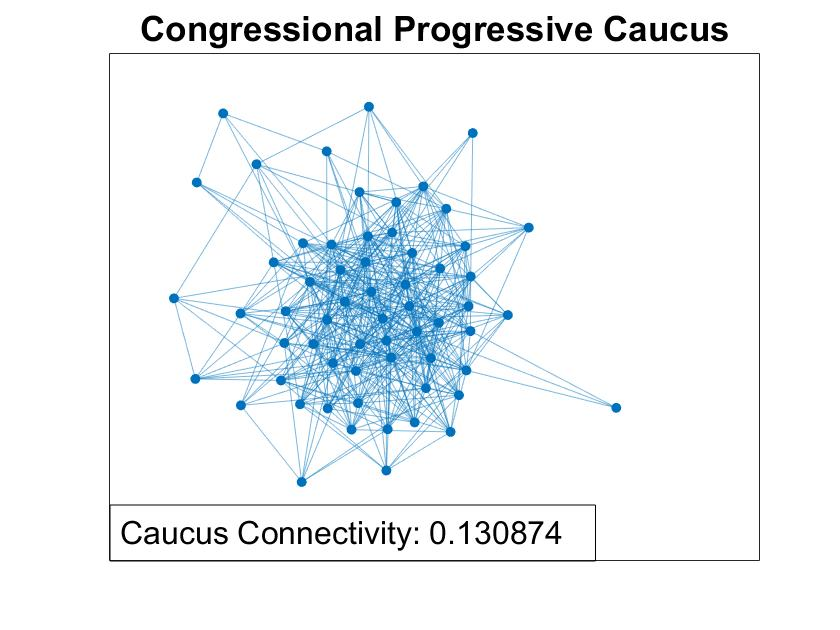
\includegraphics[width=\textwidth]{/Neighborhood_Regression/Congr_Prog_Caucus.jpg}
    \end{subfigure}
\caption{{\fontfamily{rm}\selectfont 
The connectivity is measured by the fraction of total edges present; connectivity of the whole House is 0.064.}}
\end{figure}

%\begin{figure}[h]
%  \centering
%    \subfloat{
%        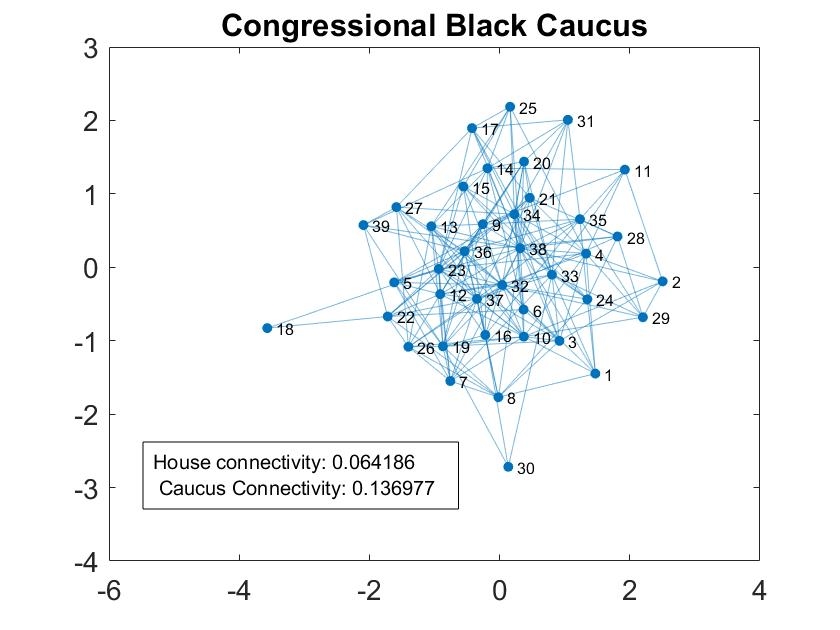
\includegraphics[width=.49\textwidth]{/Neighborhood_Regression/Congressional_Black_Caucus.jpg}}  
%        \subfloat{
%        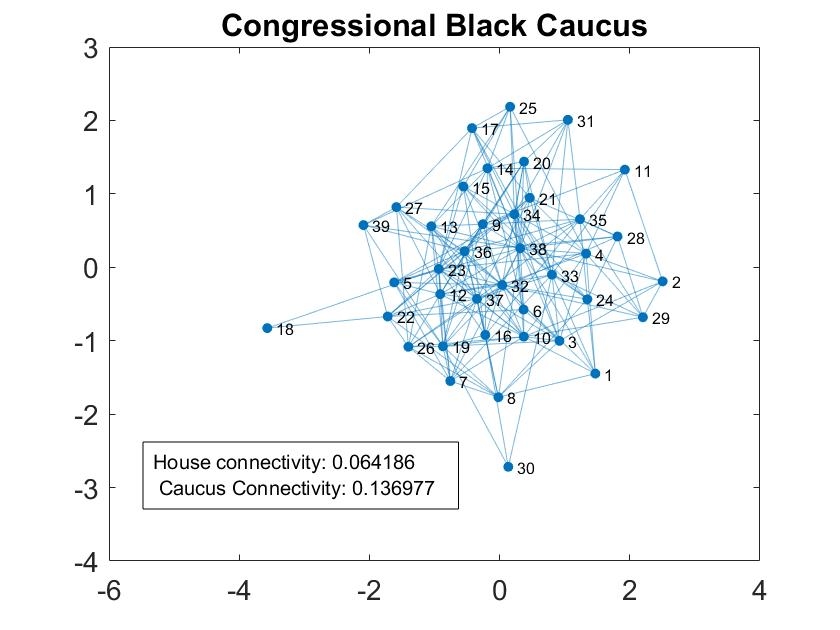
\includegraphics[width=.49\textwidth]{/Neighborhood_Regression/Congressional_Black_Caucus.jpg}}\\
%\subfloat{
%        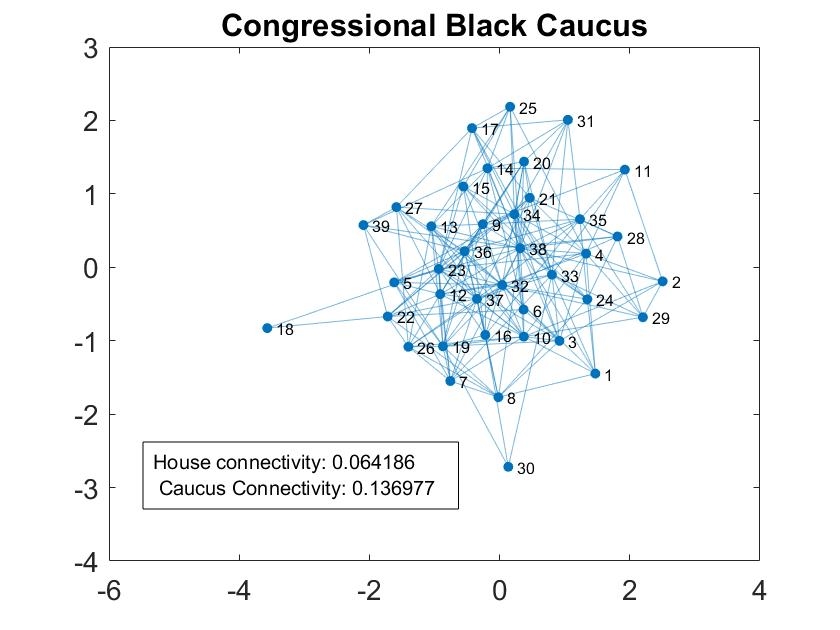
\includegraphics[width=.49\textwidth]{/Neighborhood_Regression/Congressional_Black_Caucus.jpg}}
%\subfloat{
%        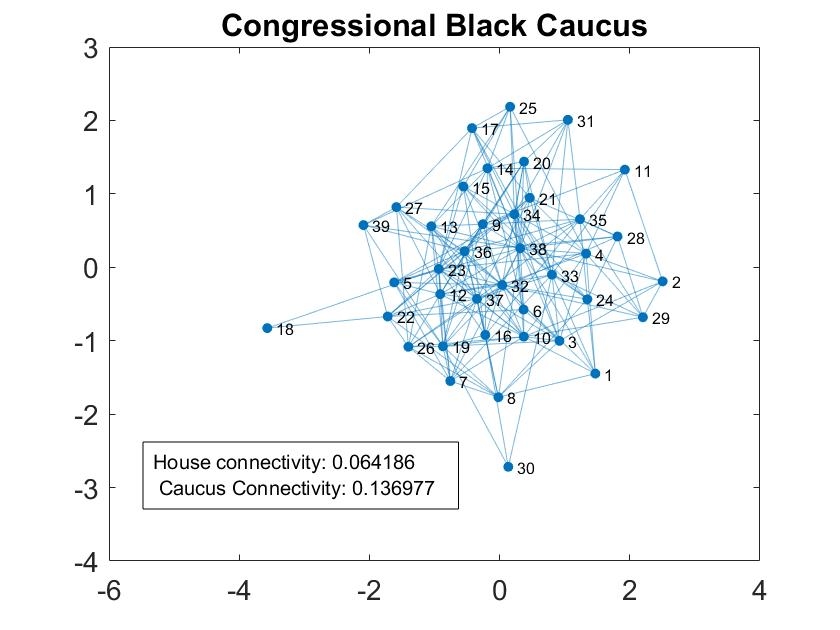
\includegraphics[width=.49\textwidth]{/Neighborhood_Regression/Congressional_Black_Caucus.jpg}}\\
%        \caption{{\fontfamily{rm}\selectfont 
%The connectivity is measured by the fraction of total edges present; connectivity of the whole House is 0.064}}
%\end{figure}
\end{block}

%------------------------------------------------


%----------------------------------------------------------------------------------------

\end{column} % End of the first column

\begin{column}{\sepwid}\end{column} % Empty spacer column

\begin{column}{\twocolwid} % Begin a column which is two columns wide (column 2)

\begin{columns}[t,totalwidth=\twocolwid] % Split up the two columns wide column

\begin{column}{\onecolwid}\vspace{-.6in} % The first column within column 2 (column 2.1)

%----------------------------------------------------------------------------------------
%	THE MODEL
%----------------------------------------------------------------------------------------

\begin{block}{Model}
Our model assumes each representative $u$ has an ideal point $x_u\in\R^S$, where $S$ is a free parameter. It also assumes each representative belongs to one of $K$ latent communities. The generative process is:
\begin{itemize}
\item Sample community proportions $\pi \sim \text{Dir}(\gamma 1_K)$ and each community ideal point $\nu_k\sim \cn_S(\varpi, \sigma^2_\nu)$
\item Draw representative $u$'s community $M_u\simiid \text{Cat}(\pi)$ and ideal point $x_u\mid M_u = k, \nu \sim \cn_S(\nu_k,\sigma^2_x)$
\item Draw coexpression rates $P_{kl} \simiid \text{Gamma}(\lambda_0,\lambda_1)$
\item Observe the number of common caucuses $R_{uv} \mid P, M_u=k, M_v=l\sim \text{Poisson}(P_{kl})$ % shared by $u$ and $v$.
\item Draw a discrimination $a_d \sim \cn_S(\eta_{a},\sigma^2_{ad})$ and a difficulty $b_d \sim \cn_S(\eta_{b},\sigma^2_{bd})$ for each bill $d$
\item Observe the votes $V_{ud} \mid x_u, a_d, b_d \sim \text{Bern}(\sigma(a_d\cdot(x_u-b_d)))$
\end{itemize}
\end{block}


%----------------------------------------------------------------------------------------

\end{column} % End of column 2.1

\begin{column}{\onecolwid}\vspace{-.6in} % The second column within column 2 (column 2.2)

\begin{figure}
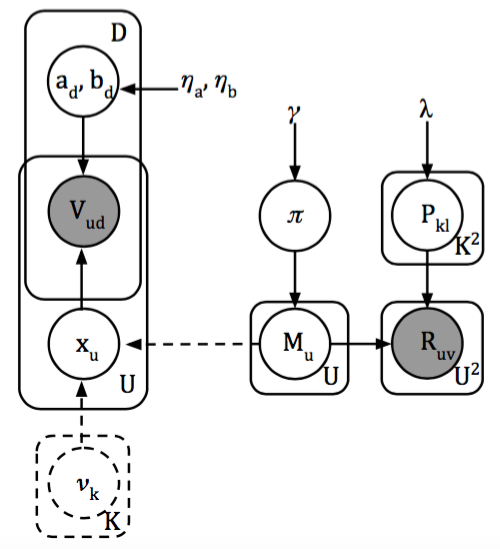
\includegraphics[width=.9\linewidth]{lcipm2.png}
\caption{{\fontfamily{rm}\selectfont Latent Community Ideal Point Model (LC-IPM)}}
\end{figure}


\end{column} % End of column 2.2

\end{columns} % End of the split of column 2 - any content after this will now take up 2 columns width

%----------------------------------------------------------------------------------------

%----------------------------------------------------------------------------------------
%	RESULTS
%----------------------------------------------------------------------------------------

\begin{block}{Results}

\begin{figure}[h]
  \centering
    \begin{subfigure}[t]{0.4\textwidth}
        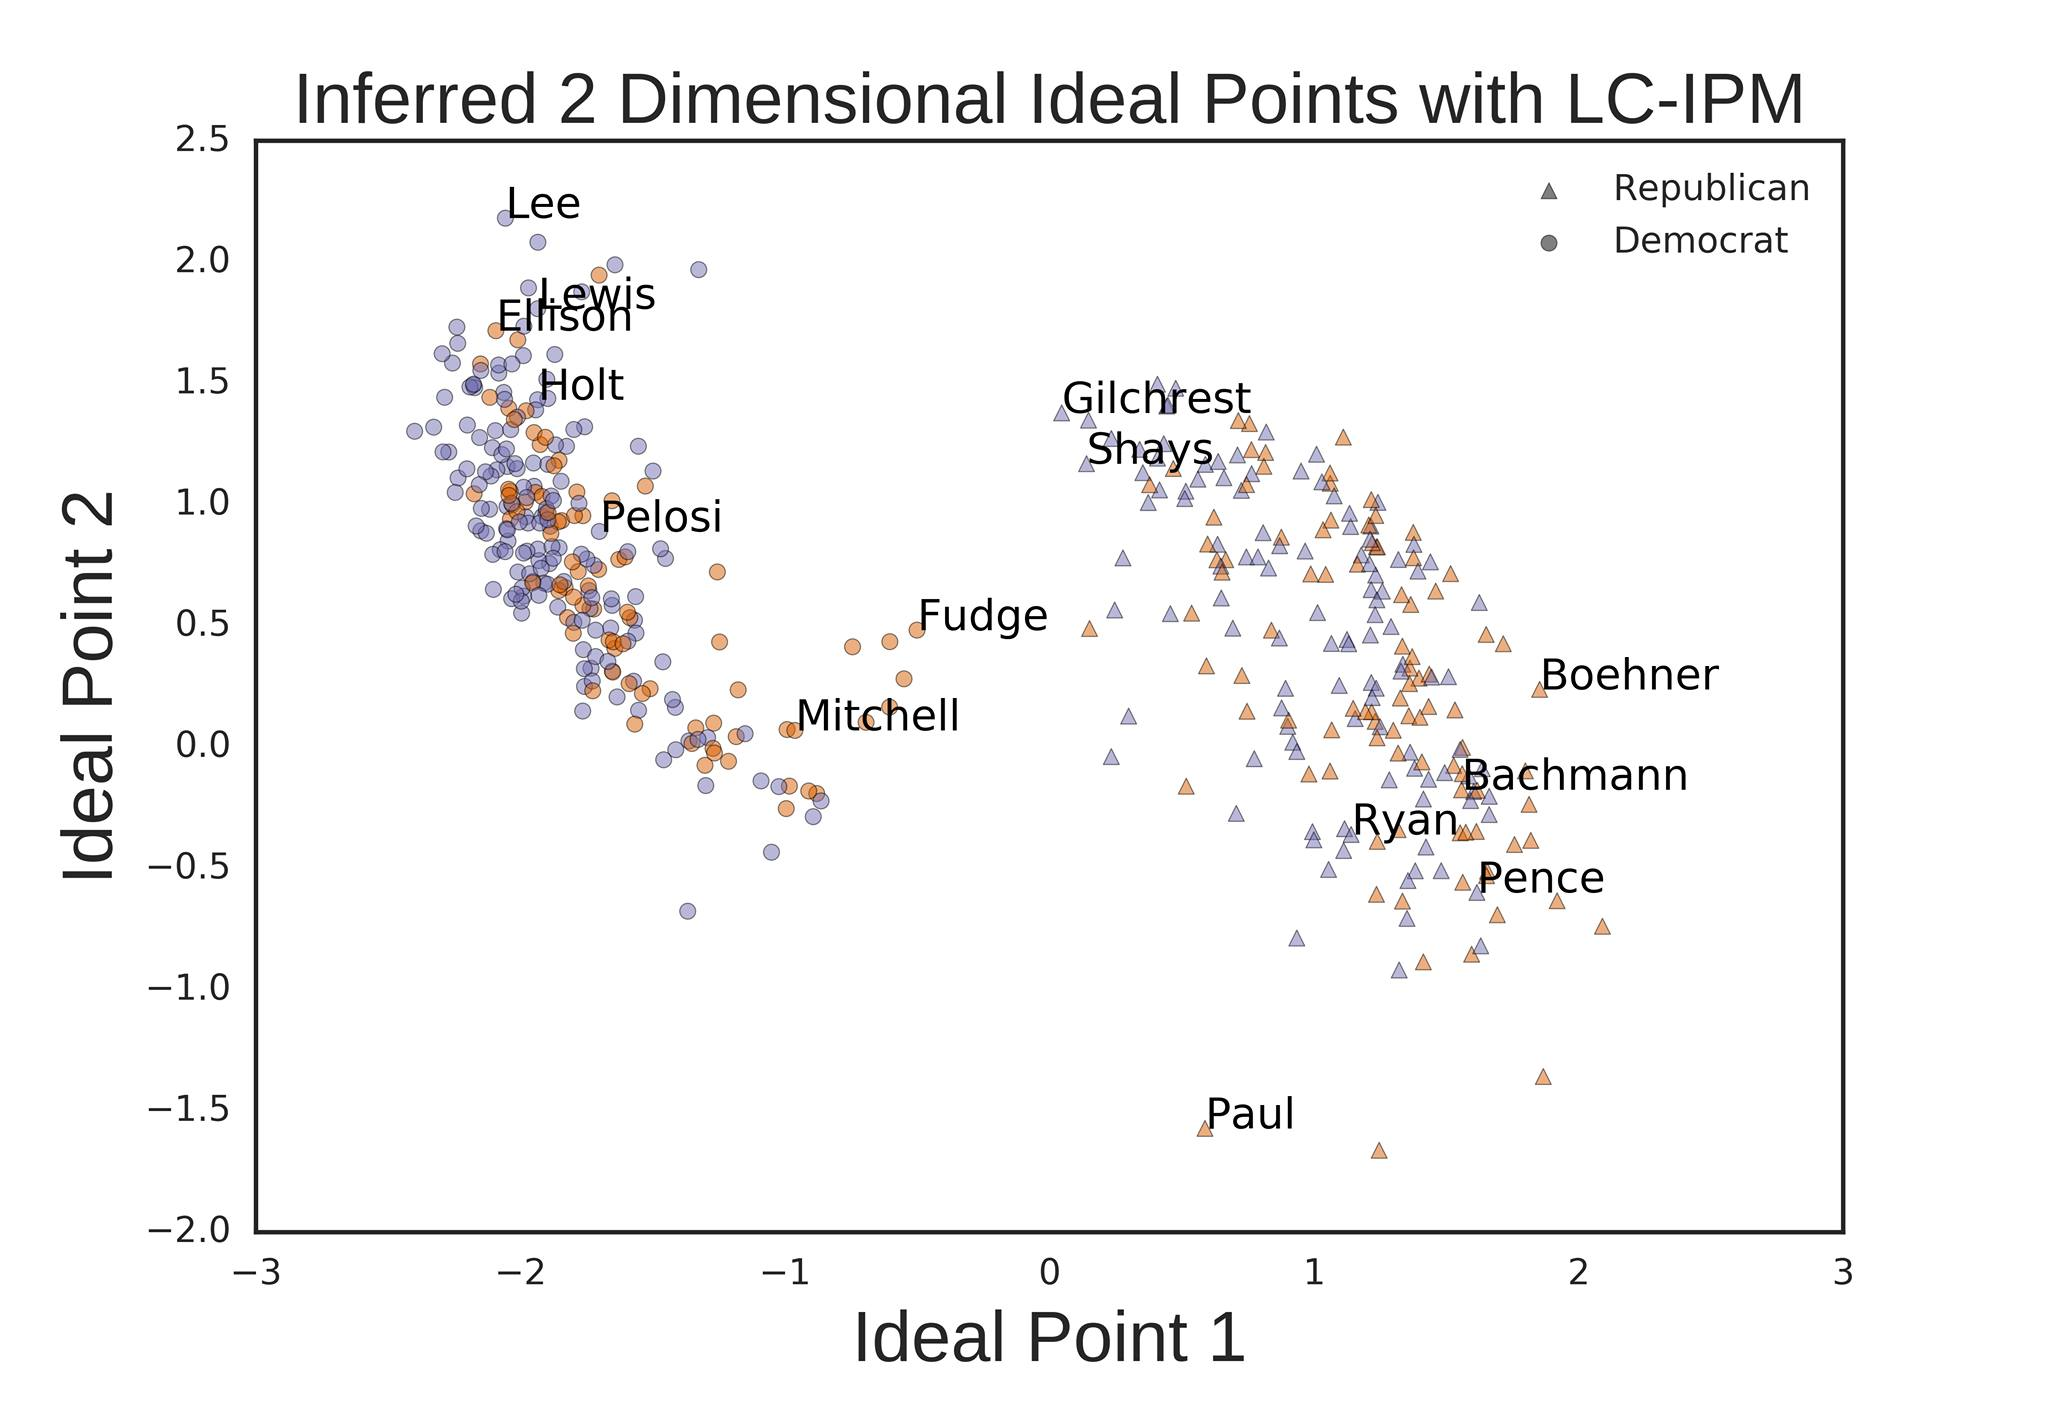
\includegraphics[width=\textwidth]{Results1.png}
        \subcaption{{\fontfamily{rm}\selectfont With $K=2$ latent communities, the inferred ideal points are well-separated by party affiliation. Shape denotes party affiliation; color denotes community.}}
    \end{subfigure}
          \begin{subfigure}[t]{0.4\textwidth}
        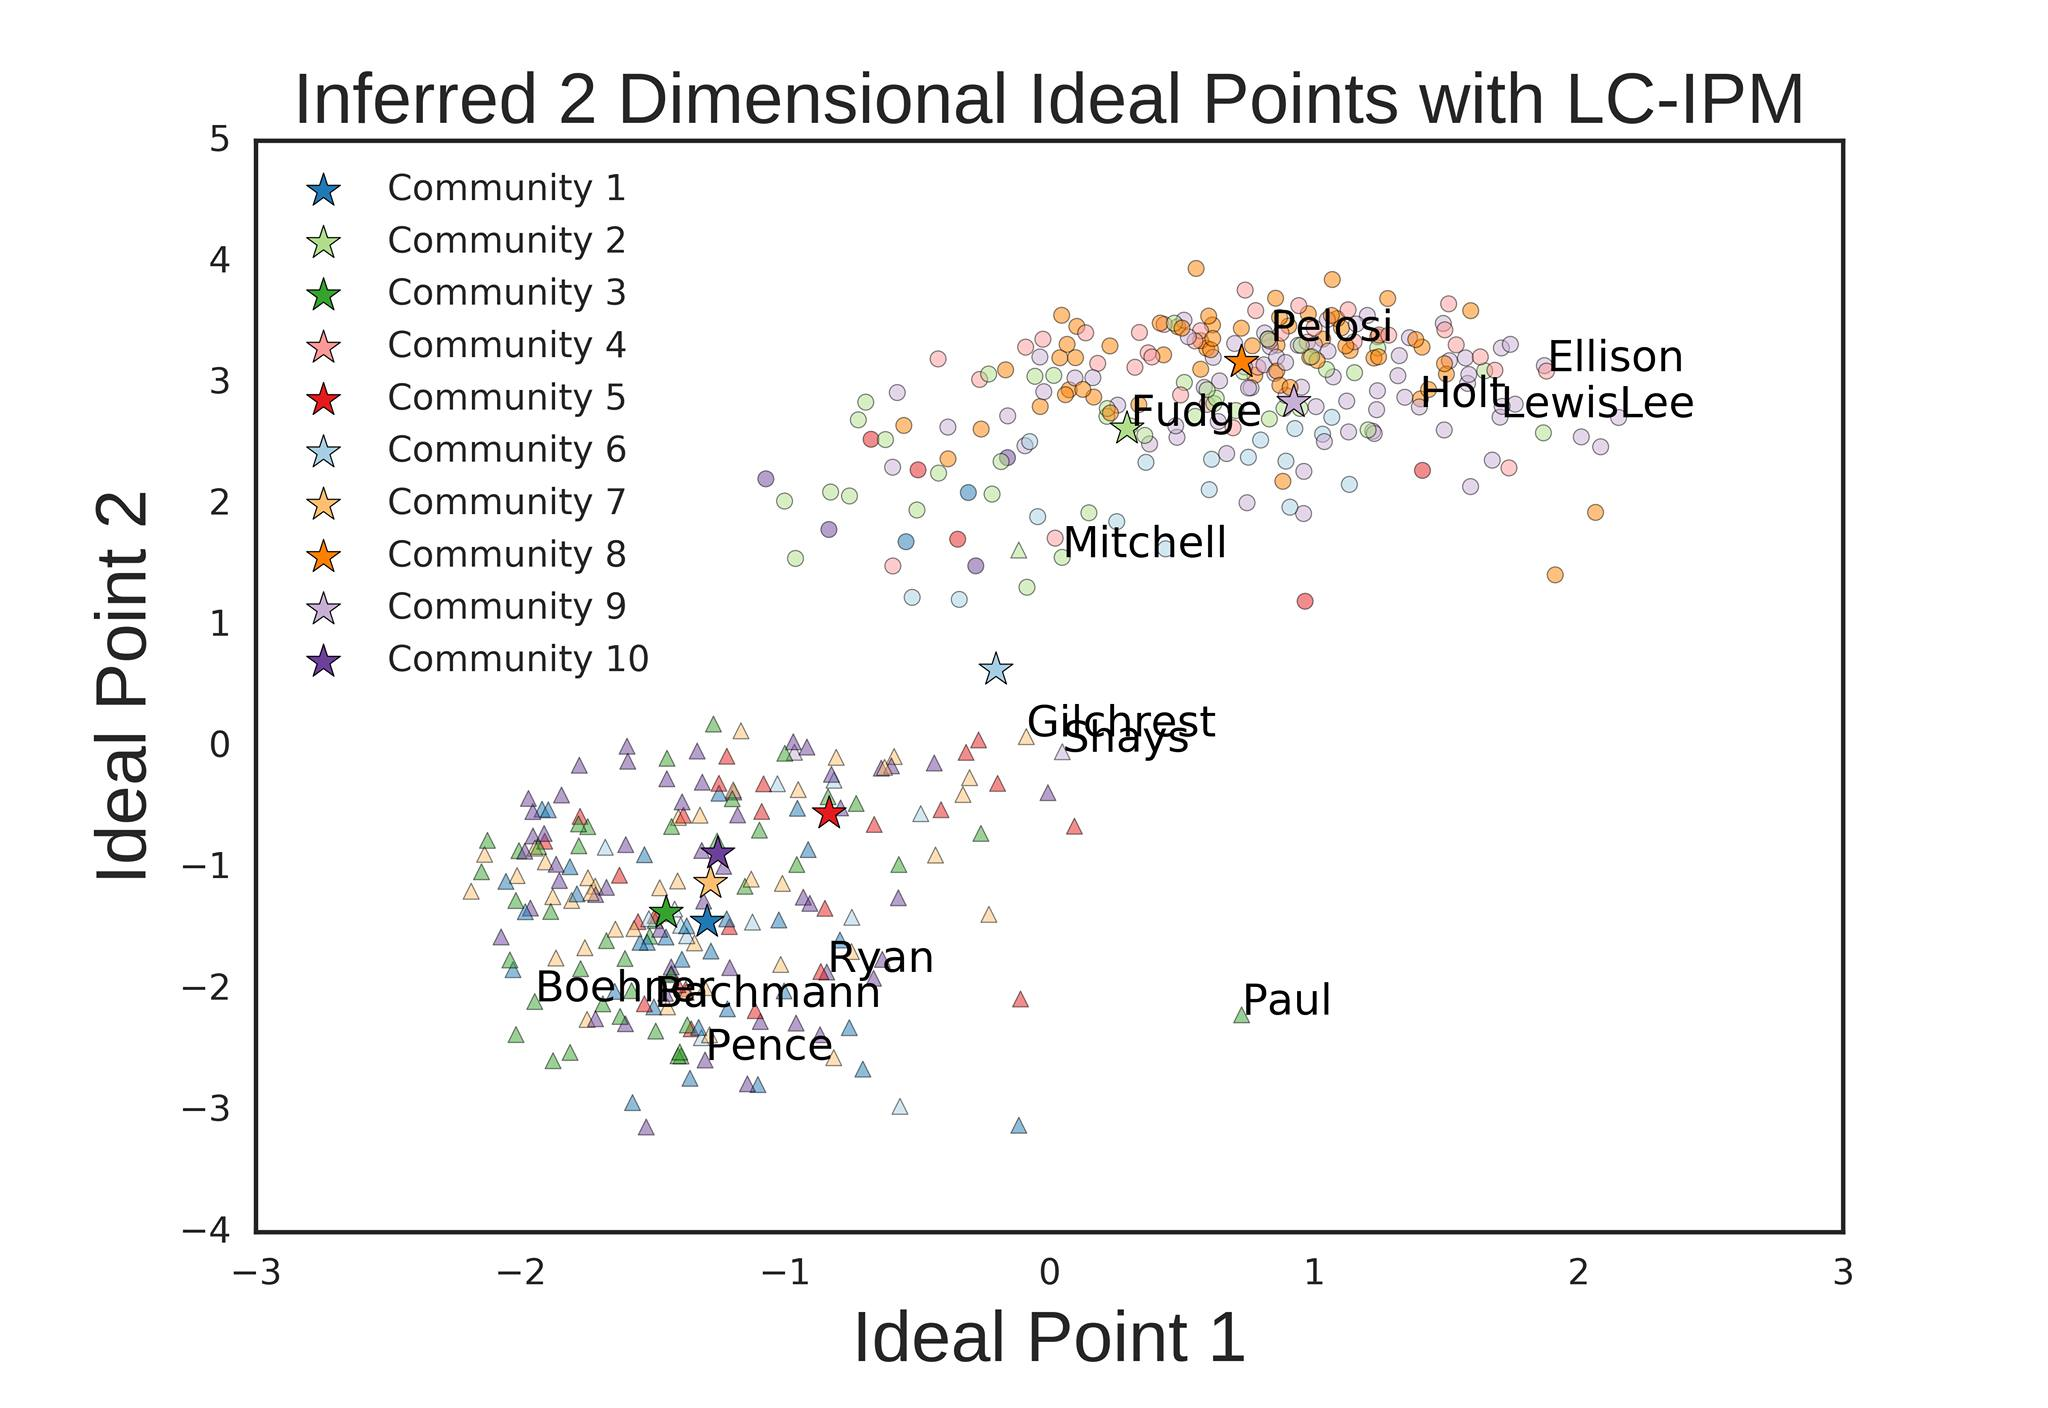
\includegraphics[width=\textwidth]{Results2.png}
        \subcaption{{\fontfamily{rm}\selectfont With $K=10$ latent communities, the inferred ideal points cluster by community, but are still well-separated by party affiliation. Shape denotes party affiliation; color denotes community.}}
    \end{subfigure}\\
        \begin{subfigure}[t]{0.4\textwidth}
        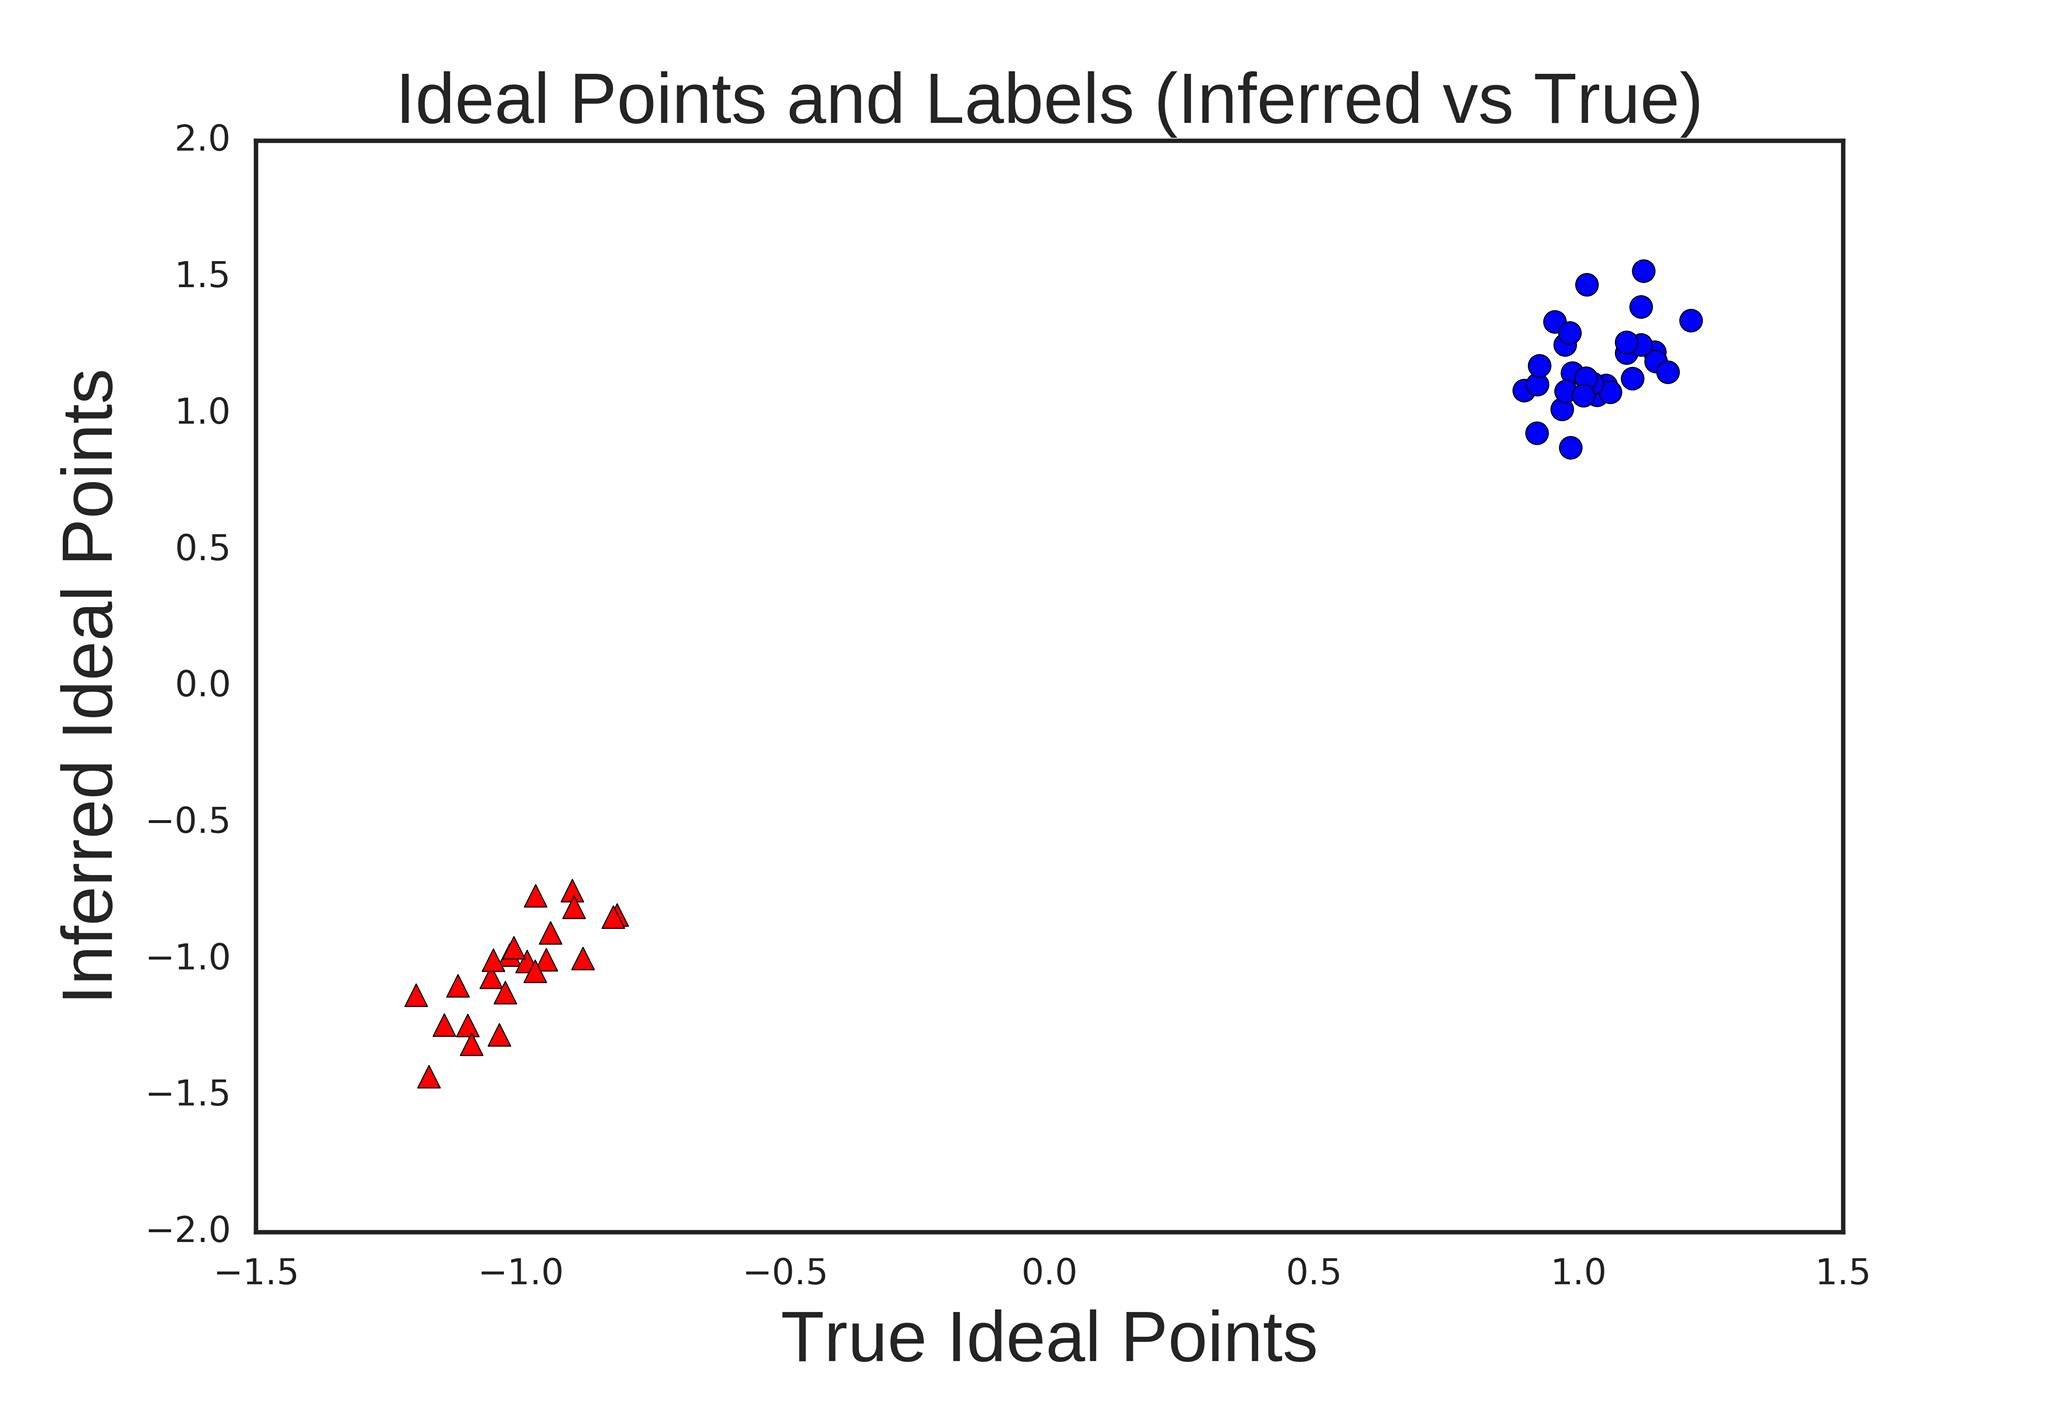
\includegraphics[width=\textwidth]{Results3.png}
        \subcaption{{\fontfamily{rm}\selectfont On toy data generated according to the graphical model, we accurately infer both the true ideal points and the community memberships. Shape denotes true community; color denotes inferred community.}}
    \end{subfigure}
          \begin{subfigure}[t]{0.4\textwidth}
        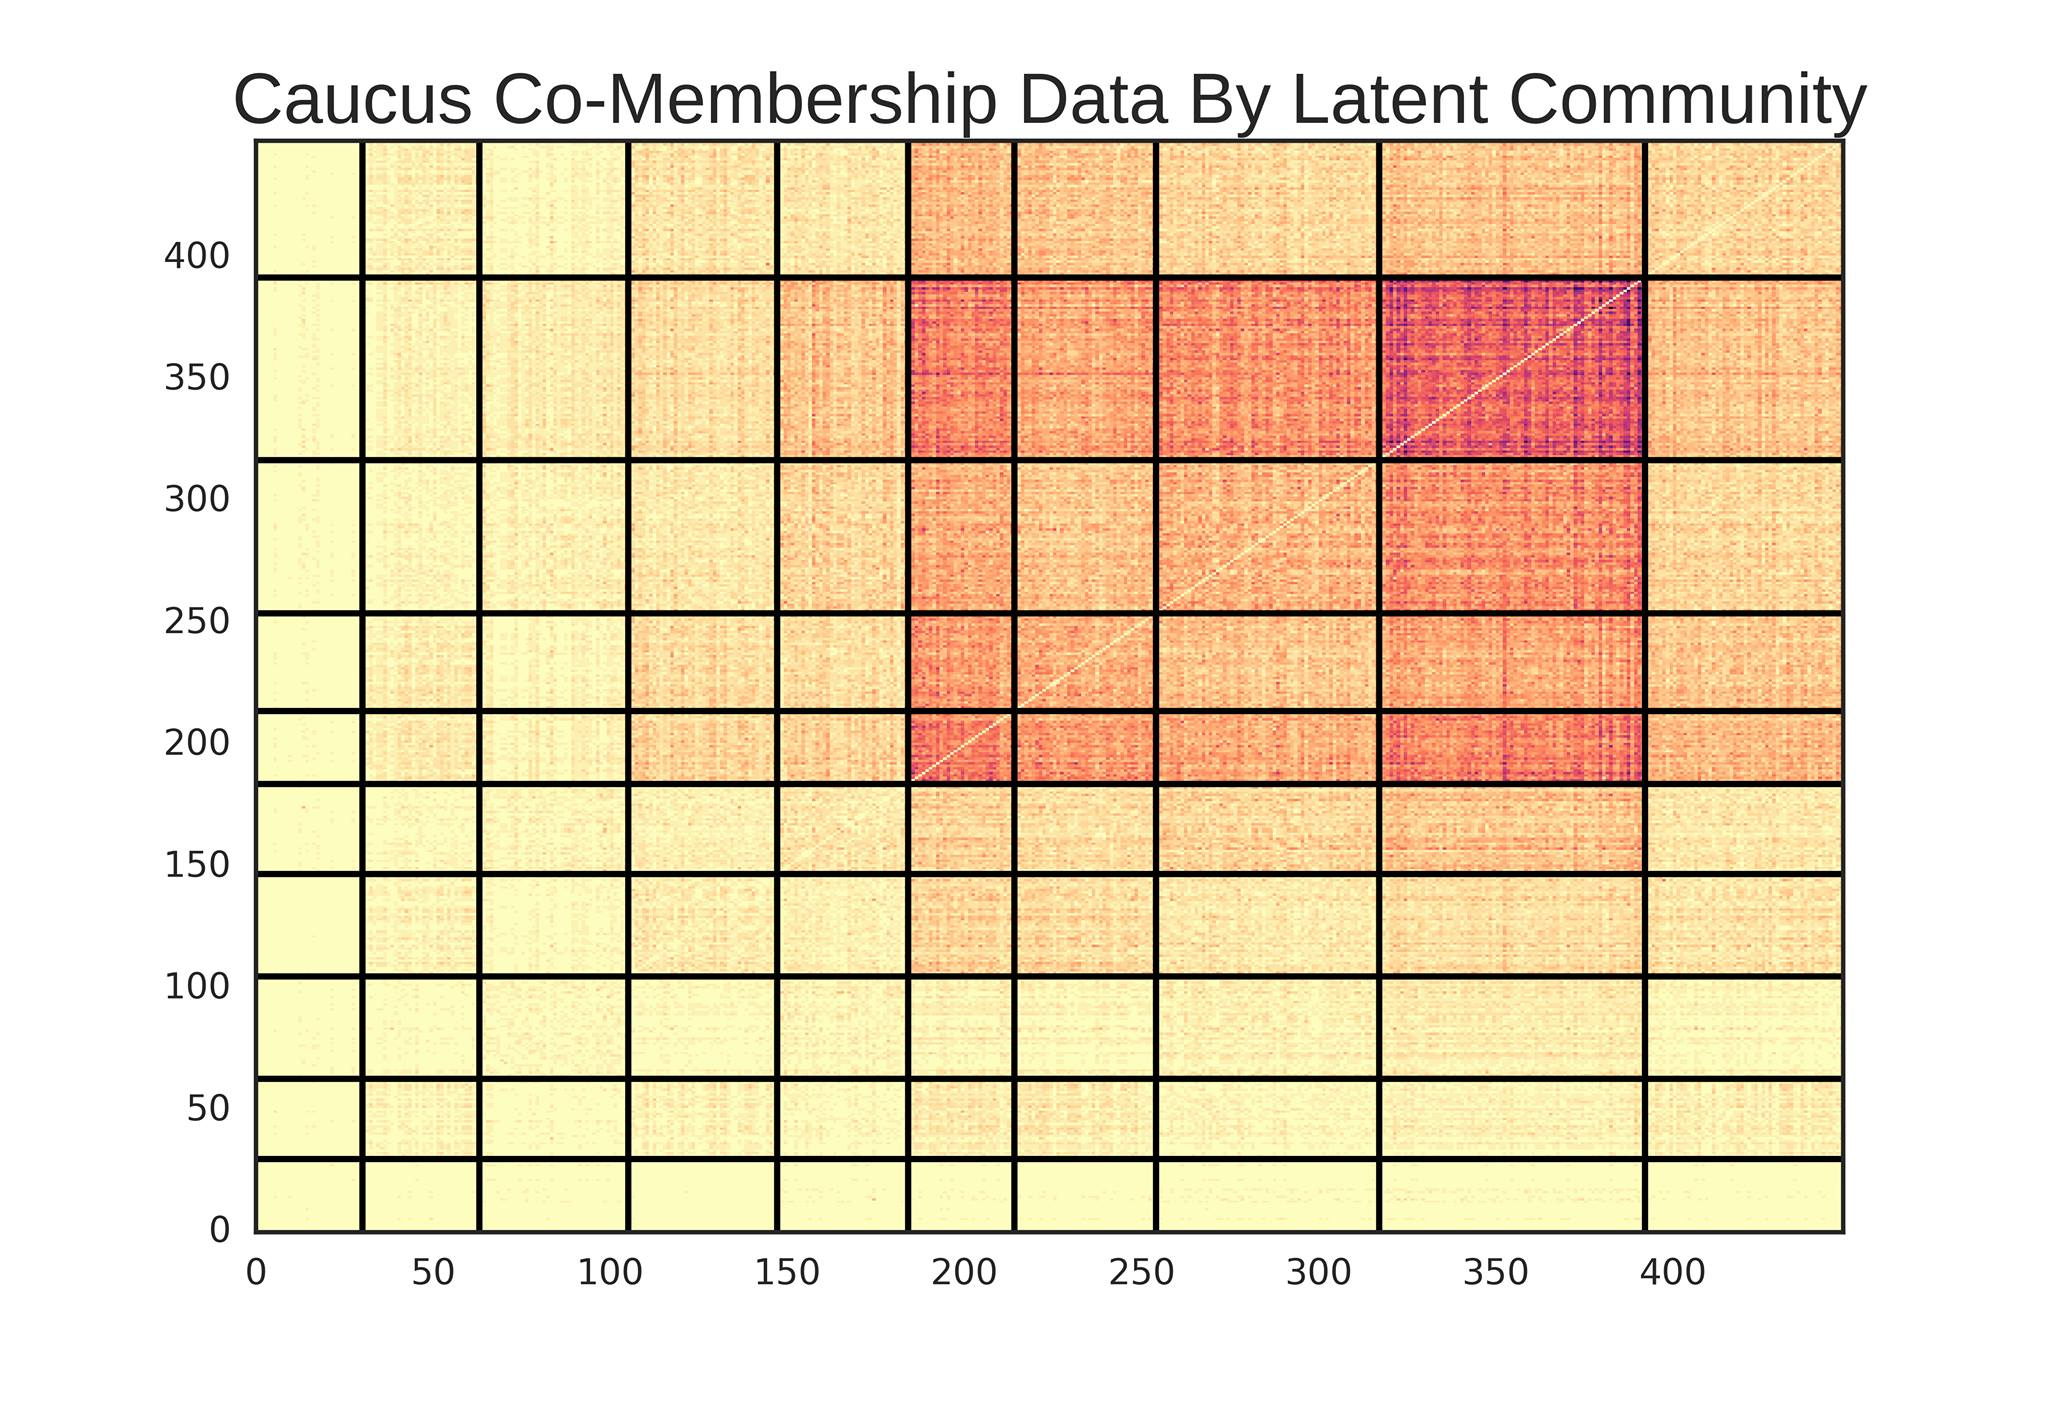
\includegraphics[width=\textwidth]{Results4.png}
        \subcaption{{\fontfamily{rm}\selectfont Each entry denotes the number of caucuses shared by a pair of representatives. Red denotes many (up to thirty) common caucuses; yellow denotes close to no common caucuses.}}
    \end{subfigure}
\end{figure}


%\begin{figure}[h]
%  \centering
%  \subfloat[][With $K=2$ latent communities, the inferred ideal points are well-separated by party affiliation. Moreover, the individuals closest to the middle of the plot are noted centrists. Shape denotes party affiliation; color denotes community. 5in.]{
%        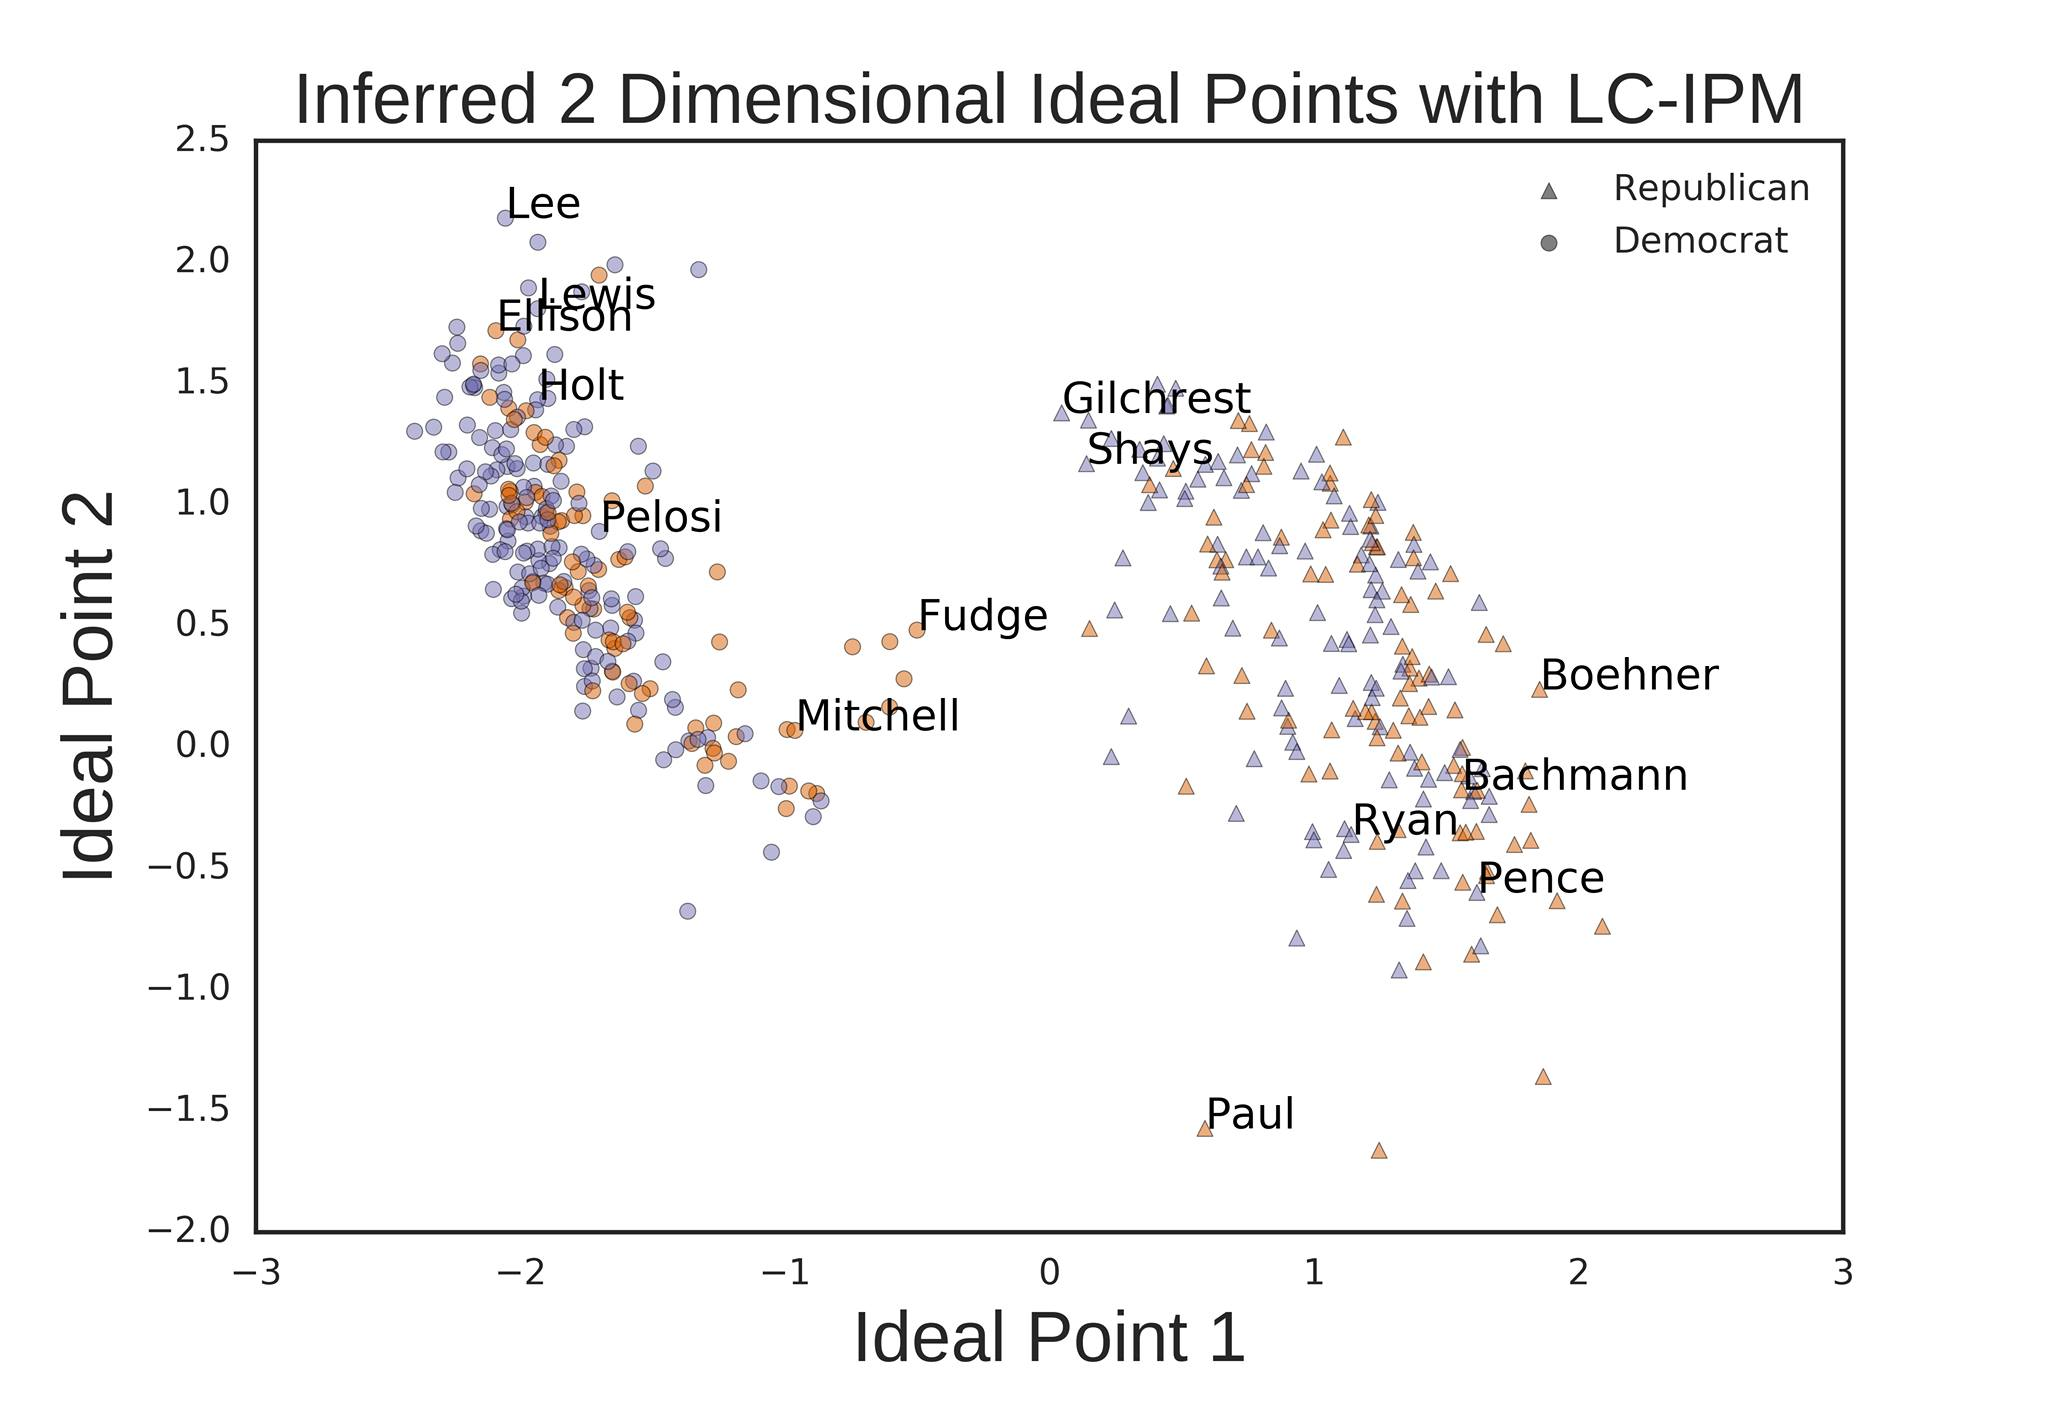
\includegraphics[width=.4\textwidth]{Results1.png}
%}
%  \subfloat[][With $K=10$ latent communities, the inferred ideal points cluster by community, but are still well-separated by party affiliation. Shape denotes party affiliation; color denotes community.]{
%        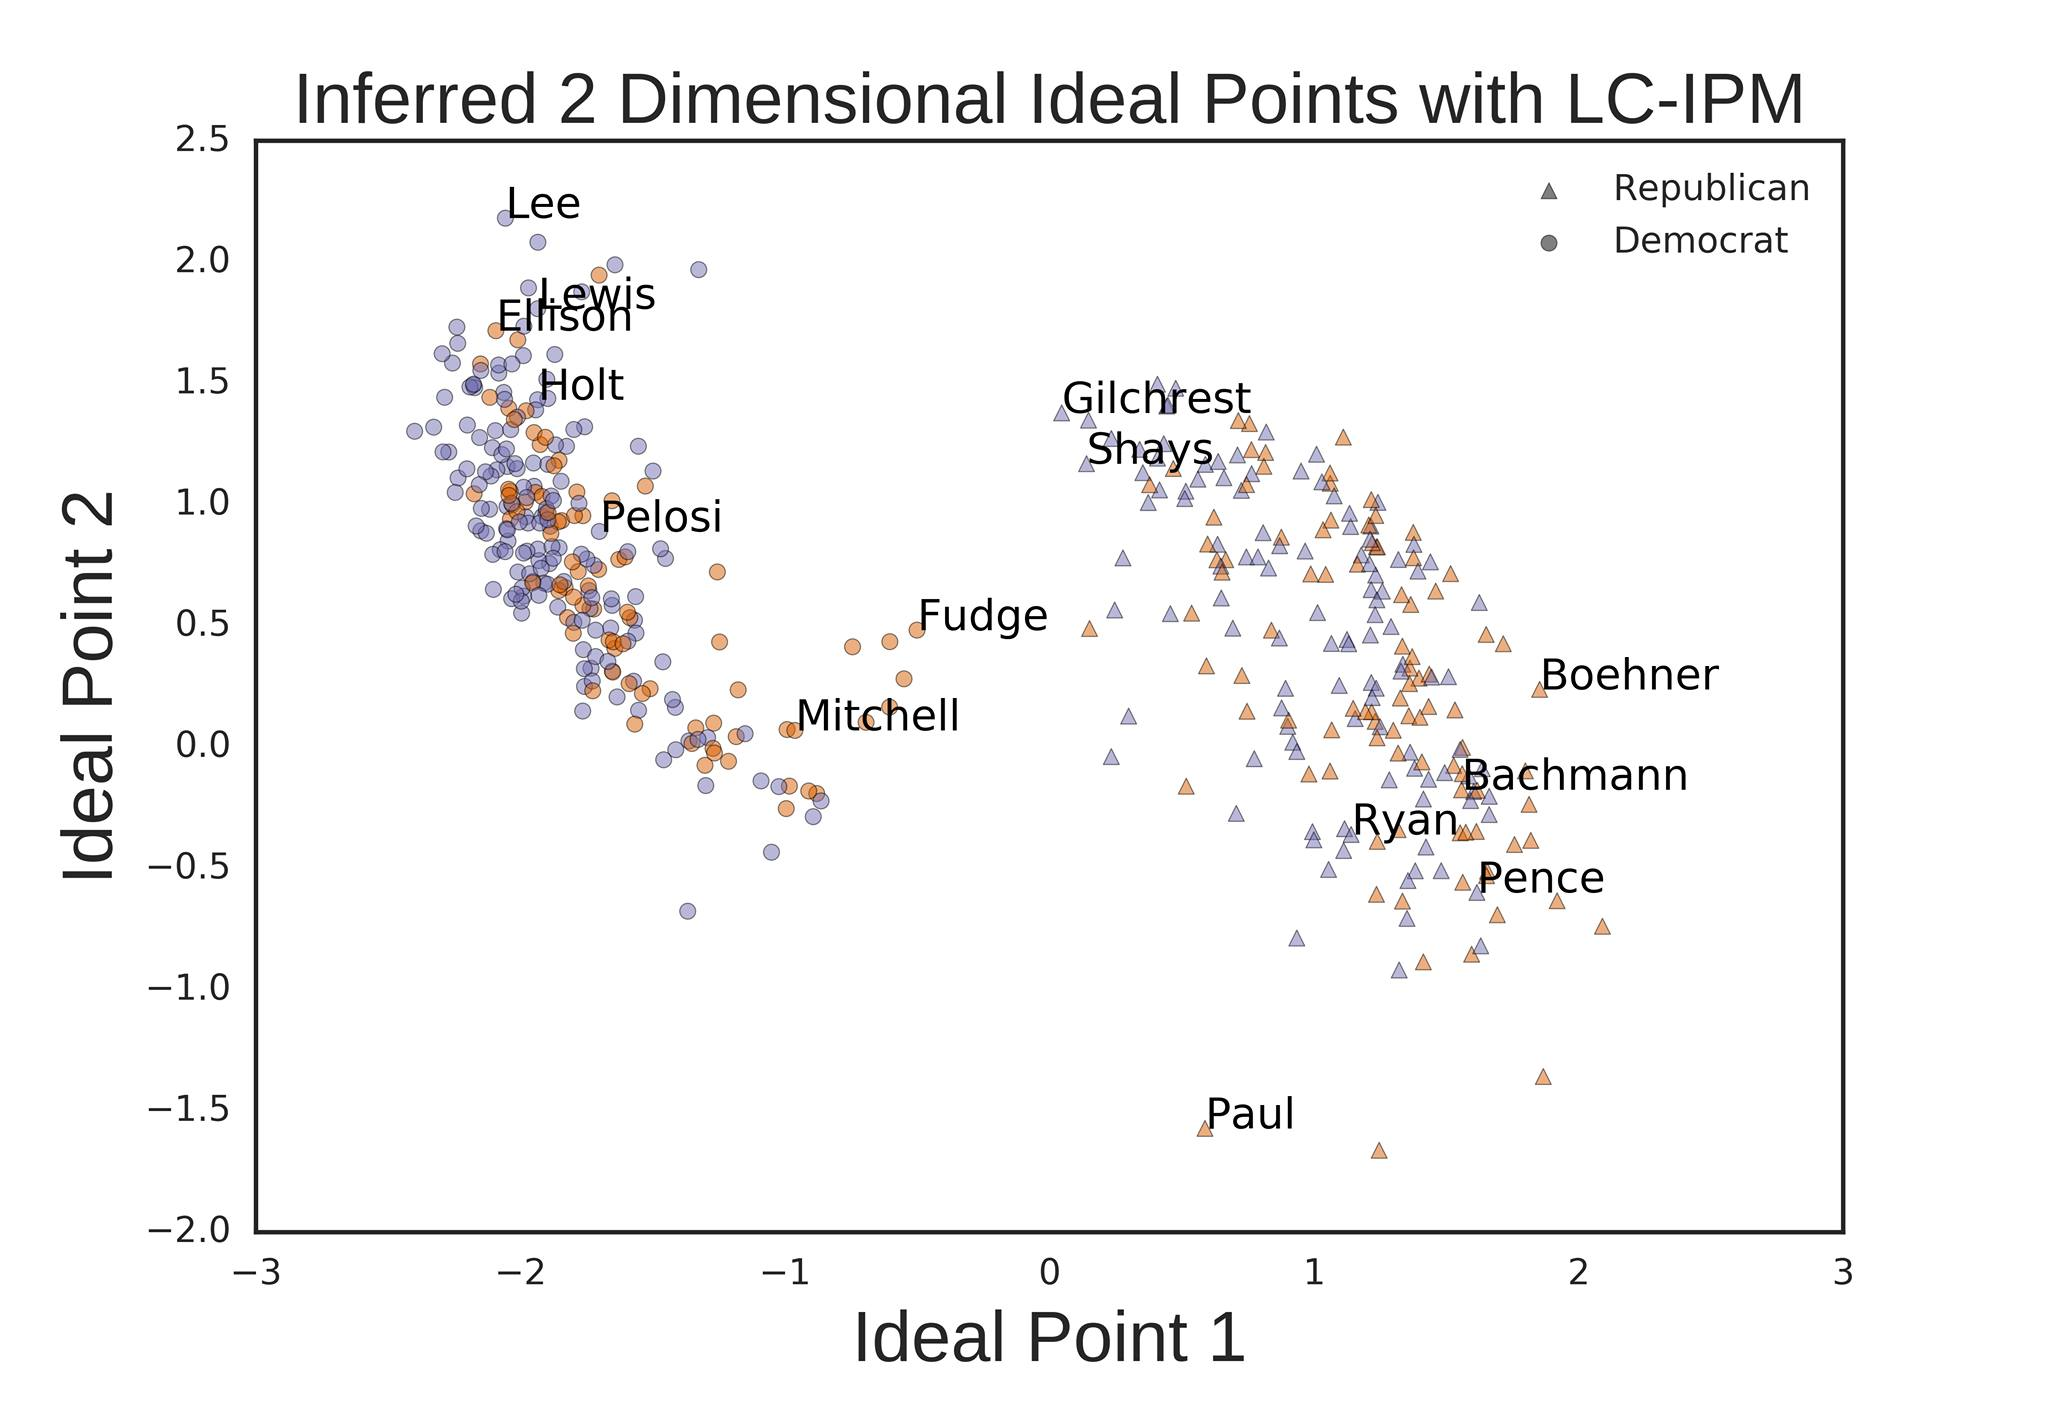
\includegraphics[width=.4\textwidth]{Results1.png}
%}\\
%  \subfloat[][On toy data generated according to the graphical model, we accurately infer both the true ideal points and the community memberships. Shape denotes true community; color denotes inferred community.]{
%        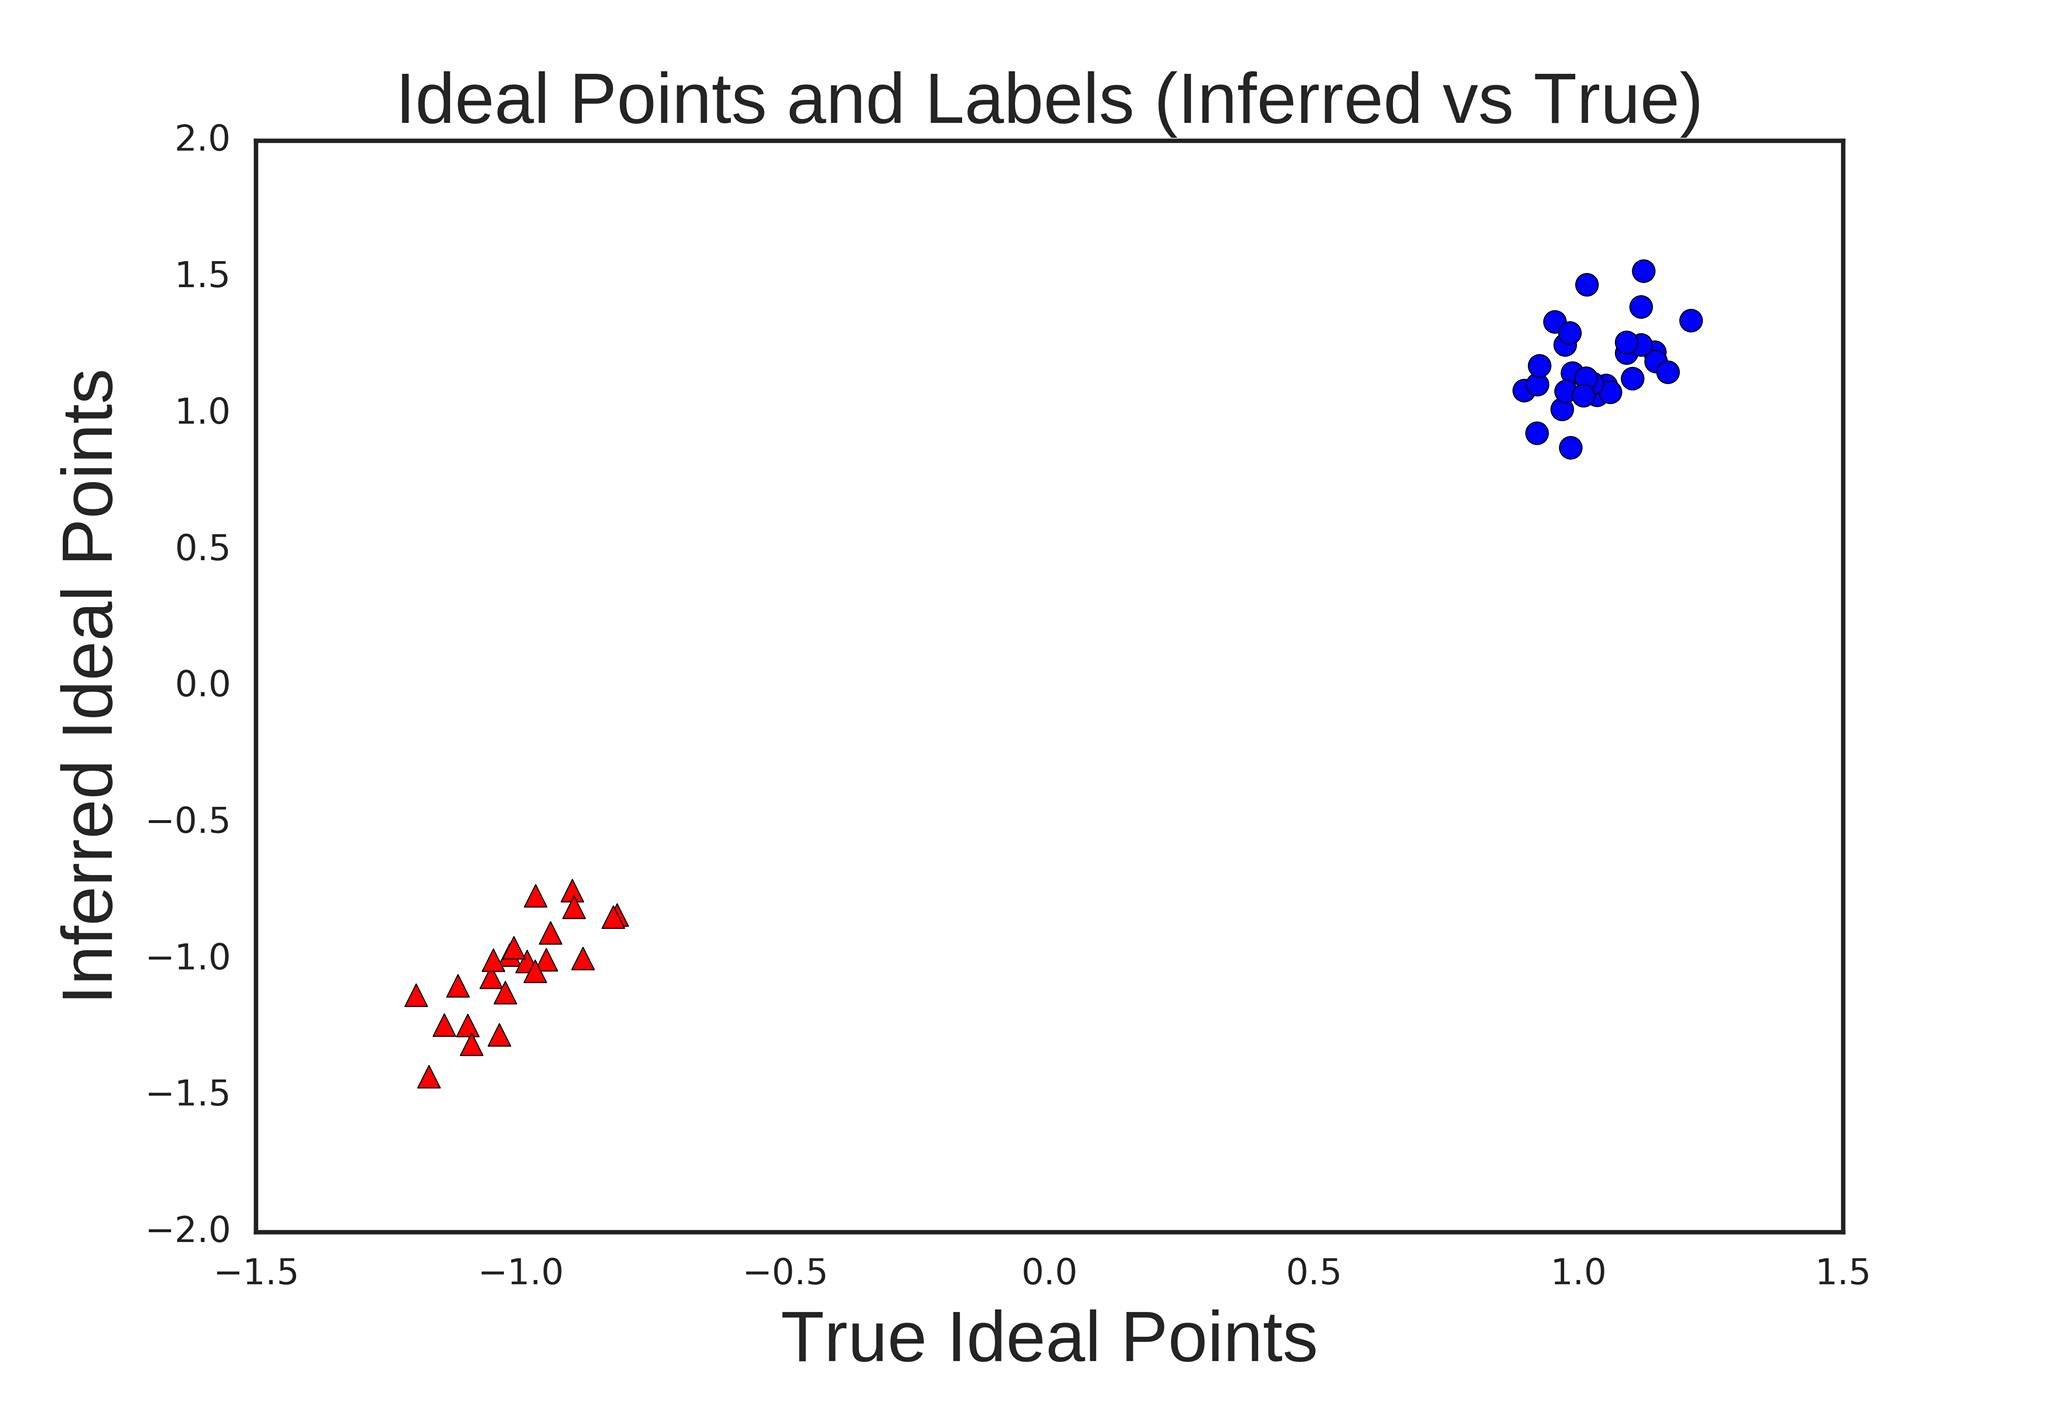
\includegraphics[width=.4\textwidth]{Results3.png}
%}
%  \subfloat[][Caucus co-membership counts grouped by inferred community. Each entry denotes the number of caucuses shared by a pair of representatives. Red denotes many (up to thirty) common caucuses; yellow denotes close to no common caucuses.]{
%        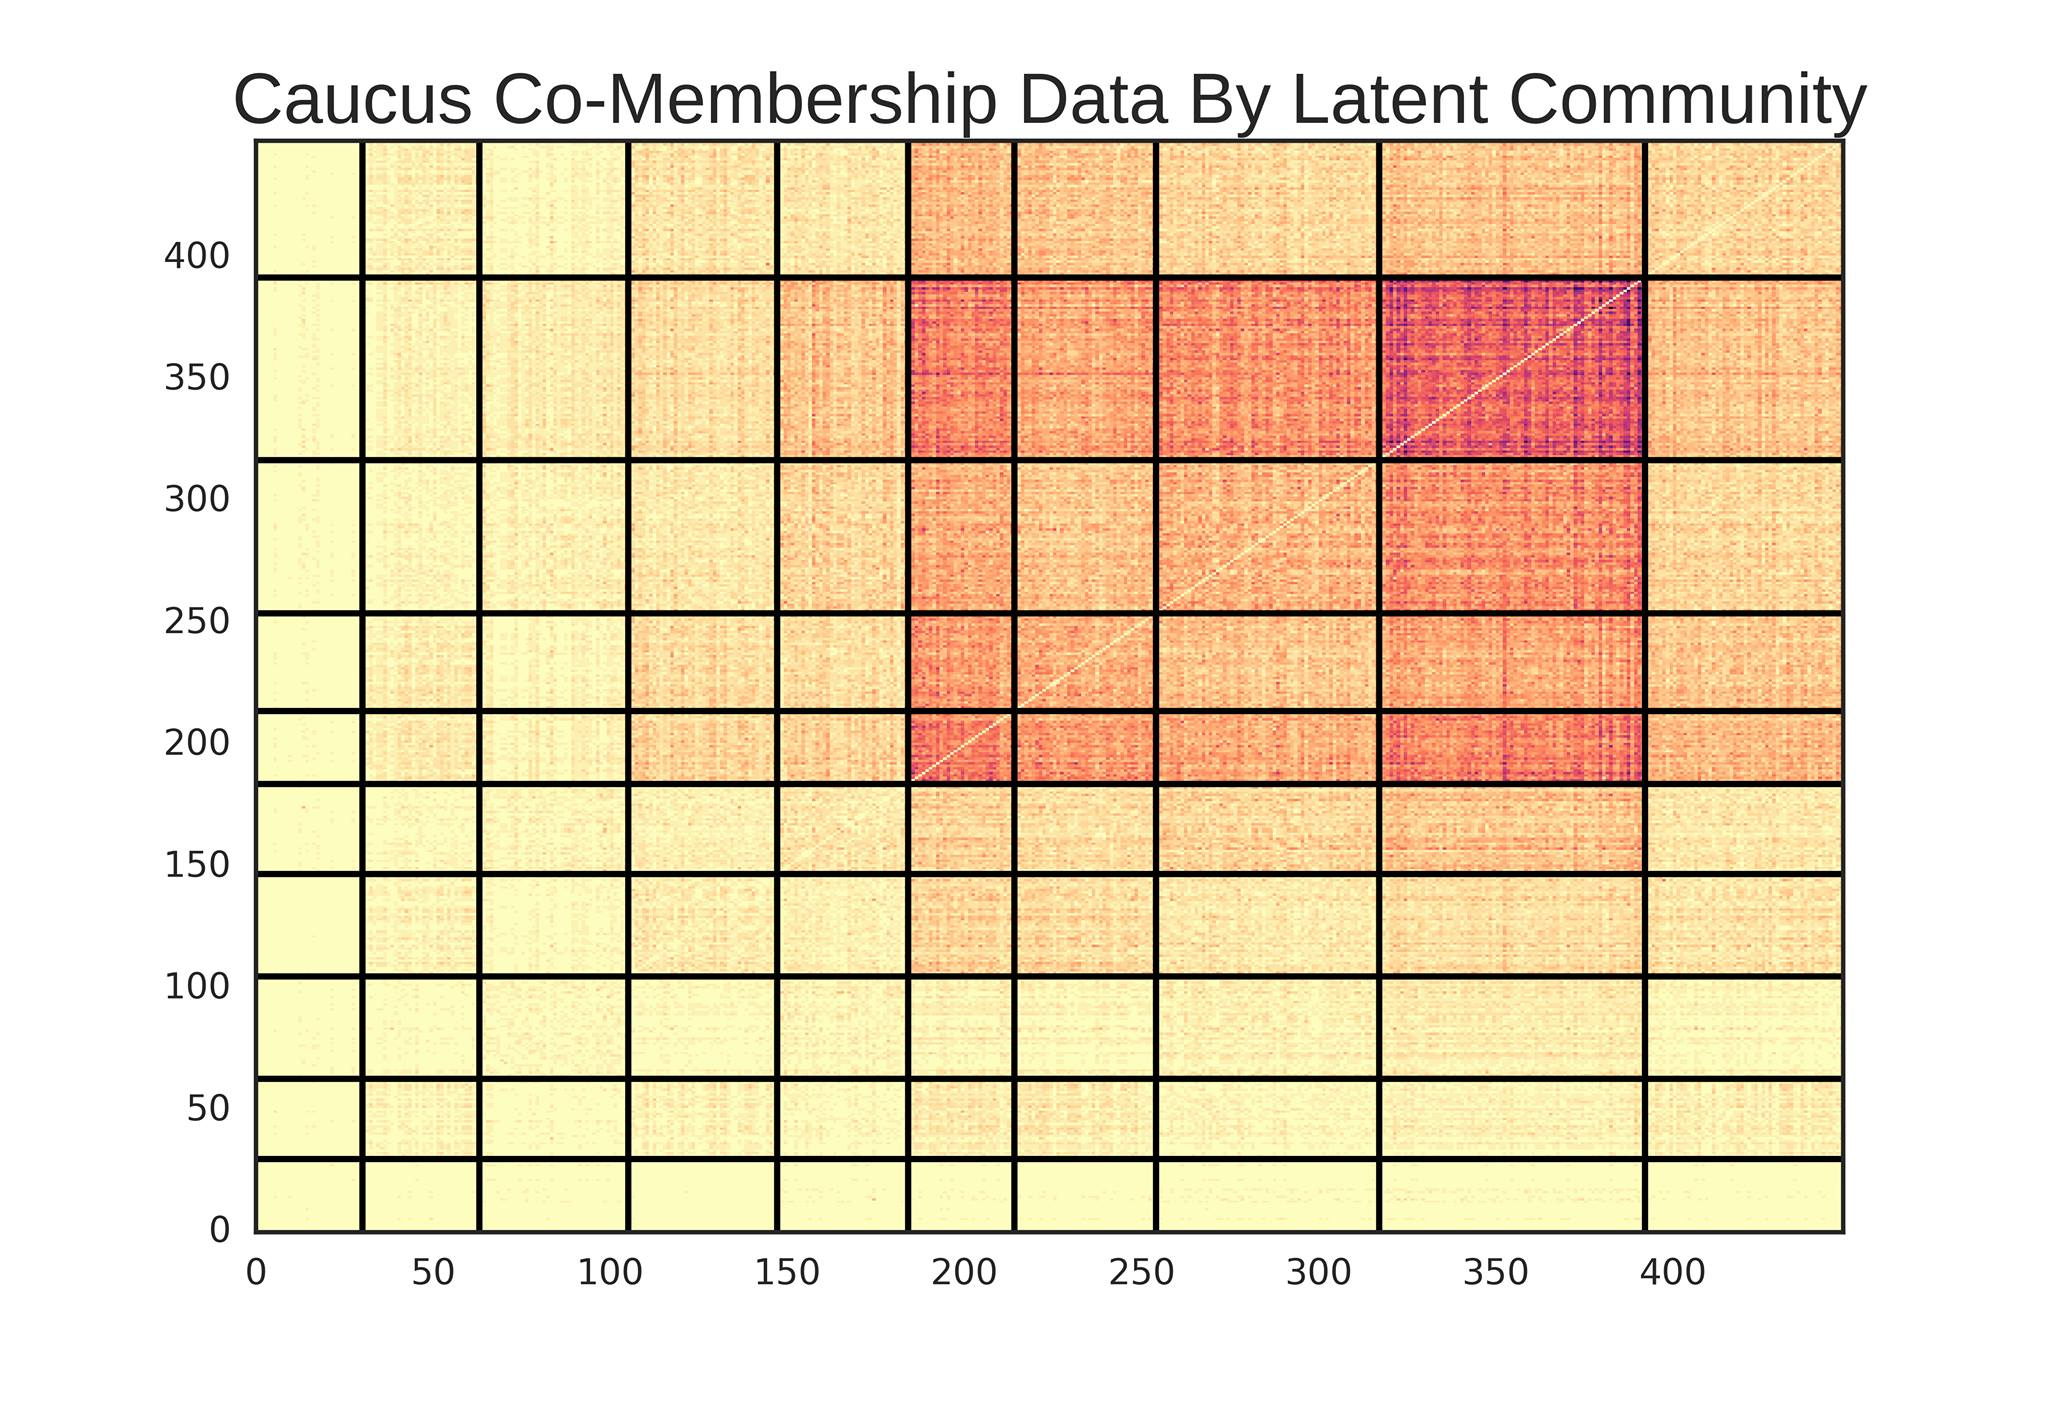
\includegraphics[width=.4\textwidth]{Results4.png}
%}

%\end{figure}

\end{block}


\end{column} % End of the second column

\begin{column}{\sepwid}\end{column} % Empty spacer column

\begin{column}{\onecolwid} % The third column

%----------------------------------------------------------------------------------------
%	Variational Inference
%----------------------------------------------------------------------------------------

\begin{block}{Variational Inference}
Upon observing votes $V = (V_{ud})$ and caucus co-memembership counts $R = (R_{uv})$, computing the posterior distribution of the latent variables given the observations is intractable. We employ {\sl mean field variational inference}, finding the distribution $q$ closest in KL divergence to the posterior among all fully factorized distributions. Since the graphical model for LC-IPM joins SBM and IPM via only one edge, the mean field factorization yields the same variational updates for $\pi, P, a_d$, and $b_d$ as in SBM and IPM, and we exploited this modularity.% in our implementation. 

\end{block}

%----------------------------------------------------------------------------------------


%----------------------------------------------------------------------------------------
%	CONCLUSION
%----------------------------------------------------------------------------------------

\begin{block}{Conclusion}

LC-IPM offers similar predictive performance to the standard ideal point model, but we gain interpretability and can make predictions for junior representatives. Our model also applies to more general collaborative filtering settings with relational data.

\begin{table}
\vspace{2ex}
\begin{table}
\begin{tabular}{c | c |c |c}
Model &  Acc & AUC\\ %$\sigma^2_x$&
\hline
\hline
Yea & 67.123 & 50.000\\
Logistic Reg & 78.340 & 85.105\\
\hline
IPM ($S= 1$)  &  94.769 & 98.418\\
IPM ($S= 2$)  & 95.451 & 98.998\\
\hline
%LC-IPM & 1 & 1 & 94.759033& 98.439207\\
%LC-IPM & 1 & 2  & 95.463571& 99.011618\\
%LC-IPM & 2 & 1  & 94.749798& 98.420599\\
LC-IPM ($S=2, K=2$)  & 95.405 & 99.013\\
LC-IPM ($S=2, K=10$)  & 95.415 & 99.015
%LC-IPM & 3 & 1  & 94.713745& 98.400689\\
%LC-IPM & 3 & 2  & 95.432136& 99.000409\\
%LC-IPM & 4 & 1  & 94.806629& 98.454243\\
%LC-IPM & 4 & 2  & 95.420414& 99.007798\\
%LC-IPM & 10 & 1  & 94.764538& 98.421727\\
%LC-IPM & 10 & 2  & 95.443324& 99.018565\\
%\hline
%LC-IPM & 2 & 2 & 0.01 & 95.265902& 98.957617\\
%LC-IPM & 2 & 2 & 0.1 & 95.413843& 99.01655\\
%LC-IPM & 2 & 2 & 100 & 95.426808& 98.99048\\
\end{tabular}
\end{table}

\end{table}

\end{block}

%----------------------------------------------------------------------------------------
%	Future Directions
%----------------------------------------------------------------------------------------

\begin{block}{Future Directions}
%By incorporating caucus data, we were able to place more informative priors on the representatives ideal points. On the other hand, we may also wish to place similarly informed priors on a bill's difficulty and discrimination. 
Following the example of [2], we hope to combine LC-IPM with {\itshape supervised topic modeling} to incorporate text data such as bill text and speeches. We are also interested in the composability of hierarchical models for multiple data sources. 
%and infer the latent topics in a bill from a bill's text; these latent topics then generate a bill's difficulty and discrimination. 


\end{block}

%----------------------------------------------------------------------------------------
%	REFERENCES
%----------------------------------------------------------------------------------------

\begin{block}{References}

%\nocite{*} % Insert publications even if they are not cited in the poster
%\small{\bibliographystyle{unsrt}
%\bibliography{bibliography}\vspace{0.75in}}
\tiny{

\noindent[1] Wainwright, M. J. \& Jordan, M. I. (2008). Graphical models, exponential families, and variational inference. {\itshape Foundations and Trends in Machine Learning}. \\

\noindent[2] Gerrish, S. M. \& Blei, D. M. (2011). Predicting legislative roll calls from text. {\itshape Proceedings of the 28th International Conference on Machine Learning}. \\

\noindent[3] Blei, D. M., Kucukelbir, A. \& McAuliffe, J. D. (2016). Variational inference: a review for statisticians. {\itshape arXiv:1601.00670}.

\noindent[4] Hasite, T. J., Tibshirani, R. \& Wainwright, M. J. (2015). Statistical learning with sparsity: the Lasso and generalizations. {\itshape CRC Press}. 
}
\end{block}

%----------------------------------------------------------------------------------------
%	ACKNOWLEDGEMENTS
%----------------------------------------------------------------------------------------

%\setbeamercolor{block title}{fg=red,bg=white} % Change the block title color
%
%\begin{block}{Acknowledgements}
%
%\small{\rmfamily{Nam mollis tristique neque eu luctus. Suspendisse rutrum congue nisi sed convallis. Aenean id neque dolor. Pellentesque habitant morbi tristique senectus et netus et malesuada fames ac turpis egestas.}} \\
%
%\end{block}

%----------------------------------------------------------------------------------------
%	CONTACT INFORMATION
%----------------------------------------------------------------------------------------

%\setbeamercolor{block alerted title}{fg=black,bg=norange} % Change the alert block title colors
%\setbeamercolor{block alerted body}{fg=black,bg=white} % Change the alert block body colors
%
%\begin{alertblock}{Contact Information}
%
%\begin{itemize}
%\item Web: \href{http://www.university.edu/smithlab}{http://www.university.edu/smithlab}
%\item Email: \href{mailto:john@smith.com}{john@smith.com}
%\item Phone: +1 (000) 111 1111
%\end{itemize}
%
%\end{alertblock}

\begin{center}
\begin{tabular}{ccc}

\includegraphics[width=.4\linewidth]{berkeleylogo.jpg} 
\end{tabular}
\end{center}

%----------------------------------------------------------------------------------------

\end{column} % End of the third column

\end{columns} % End of all the columns in the poster

\end{frame} % End of the enclosing frame

\end{document}
